%%%%%%%%%%%%%%%%%%%%%%%%%
% Dokumentinformationen %
%%%%%%%%%%%%%%%%%%%%%%%%%
\newcommand{\titleinfo}{Physik 3 - Formelsammlung}
\newcommand{\authorinfo}{Braun \& Co, J.Rast, S.K\"orner, C.Gwerder, M. Giger}
\newcommand{\versioninfo}{$Version: 1.0$}

%%%%%%%%%%%%%%%%%%%%%%%%%%%%%%%%%%%%%%%%%%%%%
% Standard projektübergreifender Header für
% - Makros 
% - Farben
% - Mathematische Operatoren
%
% DORT NUR ERGÄNZEN, NICHTS LÖSCHEN
%%%%%%%%%%%%%%%%%%%%%%%%%%%%%%%%%%%%%%%%%%%%%
% Genereller Header
\documentclass[10pt,twoside,a4paper,fleqn]{article}
\usepackage[utf8]{inputenc}
\usepackage[left=1cm,right=1cm,top=1cm,bottom=1cm,includeheadfoot]{geometry}
\usepackage[ngerman]{babel,varioref}

% Pakete
\usepackage{amssymb,amsmath,fancybox,graphicx,color,lastpage,wrapfig,fancyhdr,hyperref,verbatim}

%%%%%%%%%%
% Farben %
%%%%%%%%%%
\definecolor{black}{rgb}{0,0,0}
\definecolor{red}{rgb}{1,0,0}
\definecolor{white}{rgb}{1,1,1}
\definecolor{grey}{rgb}{0.3,0.3,0.3}
\definecolor{blue}{rgb}{0.2,0.2,0.9}

%%%%%%%%%%%%%%%%%%%%
% Generelle Makros %
%%%%%%%%%%%%%%%%%%%%
\newcommand{\kuchling}[1]{$_{\textcolor{red}{\mbox{\small{Kuchling #1}}}}$}
\newcommand{\stoecker}[1]{$_{\textcolor{grey}{\mbox{\small{Stöcker #1}}}}$}
\newcommand{\verweis}[2]{\small{(siehe auch \ref{#1}, #2 (S. \pageref{#1}))}}
\newcommand{\subsubadd}[1]{\textcolor{black}{\mbox{#1}}}

\newcommand{\grad}{\ensuremath{^\circ}}


\newcommand{\skriptsection}[2]{\section{#1 {\tiny Skript S. #2}}}
\newcommand{\skriptsubsection}[2]{\subsection{#1 {\tiny Skript S. #2}}}
\newcommand{\skriptsubsubsection}[2]{\subsubsection{#1 {\tiny Skript S. #2}}}


%%%%%%%%%%%%%%%%%%%%%%%%%%%%
% Mathematische Operatoren %
%%%%%%%%%%%%%%%%%%%%%%%%%%%%
\DeclareMathOperator{\sinc}{sinc}



% Fouriertransformationen
\unitlength1cm
\newcommand{\FT}
{
\begin{picture}(1,0.5)
\put(0.2,0.1){\circle{0.14}}\put(0.27,0.1){\line(1,0){0.5}}\put(0.77,0.1){\circle*{0.14}}
\end{picture}
}


\newcommand{\IFT}
{
\begin{picture}(1,0.5)
\put(0.2,0.1){\circle*{0.14}}\put(0.27,0.1){\line(1,0){0.45}}\put(0.77,0.1){\circle{0.14}}
\end{picture}
}



%%%%%%%%%%%%%%%%%%%%%%%%%%%%
% Allgemeine Einstellungen %
%%%%%%%%%%%%%%%%%%%%%%%%%%%%
%pdf info
\hypersetup{pdfauthor={\authorinfo},pdftitle={\titleinfo},colorlinks=false}
\author{\authorinfo}
\title{\titleinfo}

%Kopf- und Fusszeile
\pagestyle{fancy}
\fancyhf{}
%Linien oben und unten
\renewcommand{\headrulewidth}{0.5pt} 
\renewcommand{\footrulewidth}{0.5pt}

\fancyhead[L]{\titleinfo{ }\tiny{(\versioninfo)}}
%Kopfzeile rechts bzw. aussen
\fancyhead[R]{Seite \thepage { }von \pageref{LastPage}}
%Fusszeile links bzw. innen
\fancyfoot[L]{\footnotesize{\authorinfo}}
%Fusszeile rechts bzw. ausen
\fancyfoot[R]{\footnotesize{\today}}

% Einrücken verhindern versuchen
\setlength{\parindent}{0pt}

 

%Package für Grössenänderung im mathmode
\usepackage{relsize}

% Möglichst keine Ergänzungen hier, sondern in header.tex
\begin{document}
%%%%%%%%%%%%%%%%%%%%%%%%%%%%%%%%%%%%%%%%%%%%%%%%%%%%%%%%%%%%%%%%%%%%%%%%%%%%%%%%%%%%%%%%%%%%%%%%
%%%%%%%%%%%%%%%%%%%%%%%%%%%%%%%%%%%%%%%%%%%%%%%%%%%%%%%%%%%%%%%%%%%%%%%%%%%%%%%%%%%%%%%%%%%%%%%%
\section{Optik}

\subsection{Diverses}
\begin{tabular}{p{10cm}p{6cm}}
  \textbf{Wellenlängen der Spektralfarben} & \textbf{Konstanten} \\
  \begin{tabular}{|l|l|l|l|}
    \hline
      Wellenlänge in nm & Farbe & Wellenlänge in nm & Farbe \\
      \hline
      380 . . . 435 & violett  & 565 . . . 590 & gelb \\
      435 . . . 465 & blau     & 590 . . . 630 & orange \\
      465 . . . 485 & blaugrün & 630 . . . 780 & rot \\
      485 . . . 565 & grün & & \\
      \hline
  \end{tabular}
  & \textbf{Vakuumgeschwindigkeit:} \newline 
  $c=299'792'458 \frac{m}{s} \approx 3 \cdot 10^8 \frac{m}{s}$ \\
\end{tabular}

\subsection{Geometrische Optik \kuchling{360} \stoecker{309}}
\renewcommand{\arraystretch}{2}
\begin{tabular}{|p{3.5cm}|p{8.5cm}|p{6cm}|}
  \hline
  \begin{minipage}[]{3.5cm}
    Brechungsgesetz\\
    \kuchling{365} \stoecker{320}\\
  \end{minipage} &
  $\dfrac{\sin \varepsilon_1}{\sin \varepsilon_2} = \dfrac{n_2}{n_1} \qquad n_1
  \sin \varepsilon_1 = n_2 \sin \varepsilon_2 \qquad \varepsilon_1=\varepsilon_1'$ &
  \begin{minipage}[c]{5cm}
    \vspace{0.1cm}
    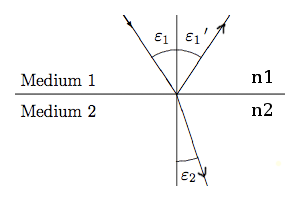
\includegraphics[width=4cm]{./bilder/Brechung.png}
  \end{minipage}\\
  \hline
  \begin{minipage}[]{3.5cm}
    \vspace{0.2cm}
    Brechungsindex\\
    \kuchling{365} \stoecker{320}\\
  \end{minipage}&
  $n=\dfrac{c}{u} \qquad$
  \begin{minipage}[]{4.5cm}
    [c]=Vakumgeschwindigkeit [u]=Lichtgeschwindigkeit
  \end{minipage} &
  \begin{minipage}[]{5cm}
    \renewcommand{\arraystretch}{1}
    \tiny
    \begin{tabular}{ l | l | l | l }
      & & & \\
      Medium & n & Medium & n \\
      \hline
      & & & \\
  		Luft   & 1,000292 & Kronglas (K13) & 1,522 \\
  		Wasser & 1,333    & Flintglas (K2) & 1,620 \\
      &          & Diamant        & 2,417 \\
    \end{tabular}
    \renewcommand{\arraystretch}{2}
  \end{minipage}\\
  \hline
  \begin{minipage}[]{3.5cm}
    Totalreflexion\\
    \kuchling{366} \stoecker{322}\\
  \end{minipage} &
  $\varepsilon = \arcsin \dfrac{n_1}{n_2} \quad$
  \begin{minipage}[]{6cm}
    $\varepsilon=\varepsilon_g \Rightarrow$ Grenzfall (ausgezogene Linie)
    $\varepsilon<\varepsilon_g \Rightarrow$ Brechung (gepunktete Linie)
    $\varepsilon>\varepsilon_g \Rightarrow$ Reflexion (gestrichelte Linie)     	
  \end{minipage} &
  \begin{minipage}[]{4cm}
    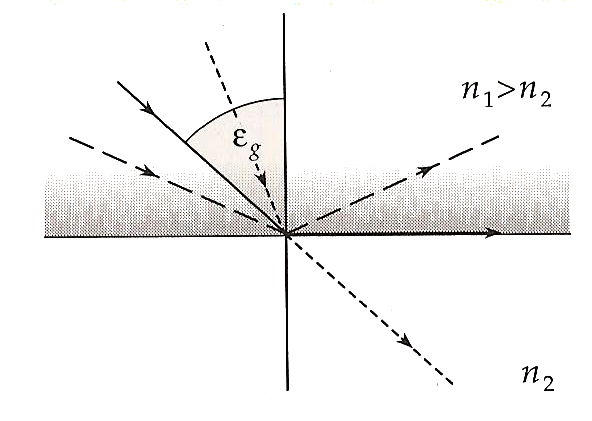
\includegraphics[width=3.5cm]{./bilder/Totalreflexion.png}
  \end{minipage}\\
  \hline
  \begin{minipage}[]{3.5cm}
    \vspace{0.2cm}
    Brennweite\\
    \kuchling{362} \stoecker{316}\\
  \end{minipage} &
  \begin{minipage}[]{6cm}
    Spiegel:\\
    $f=\dfrac{r}{2} \quad$ (für kleine $h$ gilt
    $a = b \approx \dfrac{r}{2}$) \\
    Linse:\\
    $\rightarrow$ Linsenschleifergleichung\\
  \end{minipage} &
  \begin{minipage}[]{6cm}
    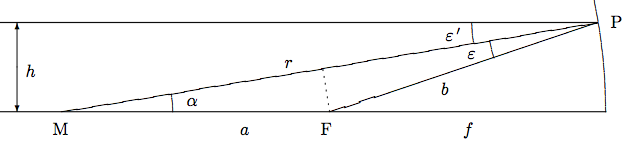
\includegraphics[width=6cm]{./bilder/BrennweiteSphaerischerSpiegel.png}
  \end{minipage}\\
  \hline
  \begin{minipage}[]{3.5cm}
    \vspace{2.7cm}
    Abbildungsgleichungen\\
    \kuchling{363} \stoecker{373}\\
  \end{minipage} &
  \begin{minipage}[c]{3cm}
    $\boxed{\dfrac{1}{f}=\dfrac{1}{g}+\dfrac{1}{b} \quad}$\\ \\
    $\boxed{\dfrac{B}{G}=\dfrac{b}{g}=\alpha}$ \\ \\
    $\boxed{\alpha_{tot} = \alpha_1 \cdot \alpha_2}$   
  \end{minipage}
  \begin{minipage}[c]{5cm}
    \vspace{0.2cm}
    G = Gegenstandshöhe\\
    g = Gegenstandsweite\\
    B = Bildhöhe\\
    b = Bildweite\\
    F = Brennpunkt\\
    f = Brennweite\\
    $\alpha$ = Vergösserungsfaktor \\
    $\alpha < 1$ = verkl., $\alpha > 1$ = vergr.\\
  \end{minipage}
  \begin{minipage}[]{8.5cm}
    \underline{Vorzeichenkonventionen}\\
    - Spiegel konkav bzw. Linse konvex $\quad \Rightarrow \quad f>0$\\
    - Spiegel konvex bzw. Linse konkav $\quad \Rightarrow \quad f<0$\\
    - Bild virtuell $\quad \Rightarrow \quad b<0 \quad\& \quad  B<0$\\
    - Gegenstand virtuell $\quad \Rightarrow \quad g<0 \quad \& \quad G<0$\\
  \end{minipage}&
  \begin{minipage}[]{6cm}
    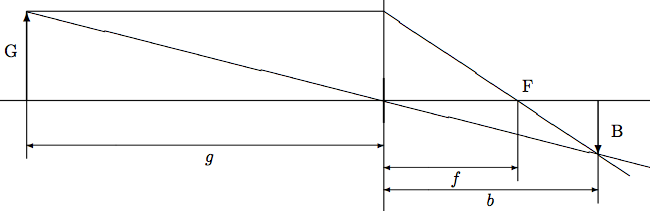
\includegraphics[width=6cm]{./bilder/Abbildungsgleichungen.png}
  \end{minipage}\\
  \hline
  \begin{minipage}[]{3.5cm}
    \vspace{0.2cm}
    Brechkraft,\\
    Linsenschleifergleichung\\
		\kuchling{370}\\
  \end{minipage} & 
  $D=\dfrac{1}{f}=\left(\dfrac{n_2}{n_1}-1\right)\left(\dfrac{1}{r_1}+
  \dfrac{1}{r_2}\right) \qquad D_{tot} = D_1 + D_2$ &
	\begin{minipage}[]{6cm}
		D = Dioptrien [dpt] \quad $1dpt=1m^{-1}$ \\
		$n_1$ = B.index d. umgebenden Mediums \\
		$n_2$ = B.index der Linse  
	\end{minipage} \\
	\hline
	Brillengleichung & $D_B = D'_{min} - D_{min} = 
	\frac{1}{g'_{min}} -\frac{1}{g_{min}}$ 
	& 
	\begin{minipage}[]{6cm}
	\vspace{0.1cm}
	 $D_B$: Dioptrien der Brille \\
	 $g'_{min}$:neue Entfernung zum Scharf sehen\\
	 $g_{min}$: alte Entfernung zum Scharf sehen \\
	 \vspace{0.1cm}
	\end{minipage} \\
	\hline
\end{tabular}

\renewcommand{\arraystretch}{1}
\newpage

\subsection{Spiegel \kuchling{362} \stoecker{315}}
\begin{minipage}[]{3.5cm}
  Konkavspiegel\\
  (Hohlspiegel)
\end{minipage}
\begin{minipage}[]{7cm}
  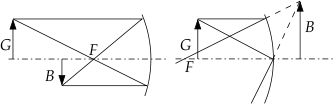
\includegraphics[width=6cm]{./bilder/Konkavspiegel.png}
\end{minipage}
\begin{minipage}[]{8cm}
  \small
  Gegenstand ausserhalb der Brennweite \\
  $\Rightarrow$ reelles, verkleinerte \& verkehrtes Bild \\ \\
  Gegenstand innerhalb der Brennweite \\
  $\Rightarrow$ virtuelles, vergrössertes \& aufrechtes Bild
\end{minipage}

\begin{minipage}[]{3.5cm}
  Konvexspiegel\\
  (Wölbspiegel)
\end{minipage}
\begin{minipage}[]{7cm}
  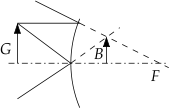
\includegraphics[width=3cm]{./bilder/Konvexspiegel.png}
\end{minipage}
\begin{minipage}[]{8cm}
  \small
  Gegenstand hat stets virtuelles, verkleinertes \& aufrechtes Bild
\end{minipage}

\begin{minipage}[]{3.5cm}
  Planspiegel
\end{minipage}
\begin{minipage}[]{7cm}
  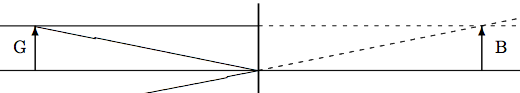
\includegraphics[height=1cm]{./bilder/Planspiegel.png}
\end{minipage}
\begin{minipage}[]{8cm}
  \small
  Bild ist virtuell und gleich gross wie Gegenstand, Bildweite ist gleich
  Gegenstandsweite. Brennpunkt liegt im Unendlichen.
\end{minipage}

\subsection{Linsen \kuchling{369} \stoecker{331}}
\begin{minipage}[]{3.5cm}
  Sammellinsen
\end{minipage}
\begin{minipage}[]{2cm}
  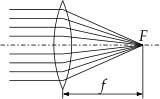
\includegraphics[width=2cm]{./bilder/sammelprinzip.png}
\end{minipage}
\begin{minipage}[]{5cm}
  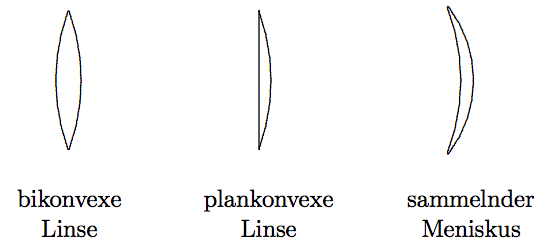
\includegraphics[width=5cm]{./bilder/sammellinsen.png}
\end{minipage}
\begin{minipage}[]{7.5cm}
  \small
  Gegenstand ausserhalb der Brennweite \\
  $\Rightarrow$ reelles, verkehrtes Bild \\ \\
  Gegenstand innerhalb der Brennweite \\
  $\quad \Rightarrow$ virtuelles, verkleinertes \& aufrechtes Bild
\end{minipage}

\begin{minipage}[]{3.5cm}
  Zerstreuungslinsen
\end{minipage}
\begin{minipage}[]{2cm}
  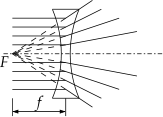
\includegraphics[width=2cm]{./bilder/streuprinzip.png}
\end{minipage}
\begin{minipage}[]{5cm}
  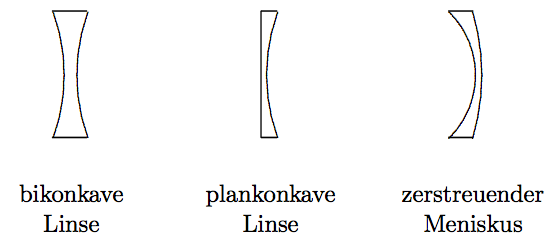
\includegraphics[width=5cm]{./bilder/streulinsen.png}
\end{minipage}
\begin{minipage}[]{7.5cm}
  \small
  Gegenstand hat stets virtuelles, aufrechtes \& verkleinertes Bild
\end{minipage}

\subsection{Abbildungsfehler}
\begin{tabular}{ll}
  Sph"arische Abberation & Brennweite ist Funktion des Abstands zur optischen
  Achse \\
  Koma & beim schiefen Einfall ($\rightarrow$ Schweiff"ormiger Fehler) \\
  Astigmatismus, Bildfeldw"olbung & vertikal und horizontal $\rightarrow$ andere
  Brennweite (Auge) \\
  Verzeichnung & tonnen- oder kissenf"ormige Verzeichnung eines Quadrates
  ($\rightarrow$ Photogrammetrie) \\
  Chromatische Abberation & wegen Dispersion $\Rightarrow$ Brennweite ist
  Funktion von $\lambda$ (Farbe) \\
\end{tabular}

\subsection{Optische Systeme}
\subsubsection{Kamera \kuchling{378} \stoecker{343}}
\begin{tabular}{lll}
  \parbox{3cm}{
    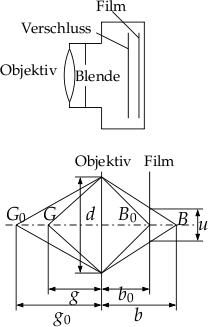
\includegraphics[width=3cm]{./bilder/kamera.png}} &
  \parbox{7cm}{
    Erzeugt reelles, verkleinertes \& umgekehrtes Bild \\
    \\
    $g \;$ Schärfentiefe\\
    $g_0 \;$ Eingestellte Entfernung (zum Gegenstand)\\
    $Z \;$ Blendenzahl \\
    $E \;$ Belichtung \\
    $u \;$ Unsch"arfekreisdurchmesser \\
    $q \;$ Öffnungsverhältnis (Blendenöffnung) \\
    $d \;$ Objektivdurchmesser \\
    $f \;$ Brennweite (z.B. 35mm-Objektiv)} &
  \parbox{8cm}{
    \fbox{$\dfrac{1}{g}=\dfrac{1}{g_0}\pm\dfrac{u}{q\,f^2}$} \\
    $B=\dfrac{f}{g-f}G$ \qquad bzw. f"ur $g\gg f\quad B=\dfrac{f}{g}G$\\
    $Z = \dfrac{f}{d} = \dfrac1q$ \qquad $q = \dfrac{d}{f} = \dfrac1Z$\\
    $E\sim q^2\,t$ \\
    Kleine Blende ($Z=16, \,q=1:16$)\\ 
    $\Rightarrow$ grosse Tiefensch"arfe\\
    Grosse Blende ($Z=4,\,q=1:4$) \\ 
    $\Rightarrow$ viel Licht, kleine Tiefensch"arfe} \\
\end{tabular}

\subsubsection{Lupe \kuchling{381} \stoecker{345}}
\begin{tabular}{lll}
  \parbox{7cm}{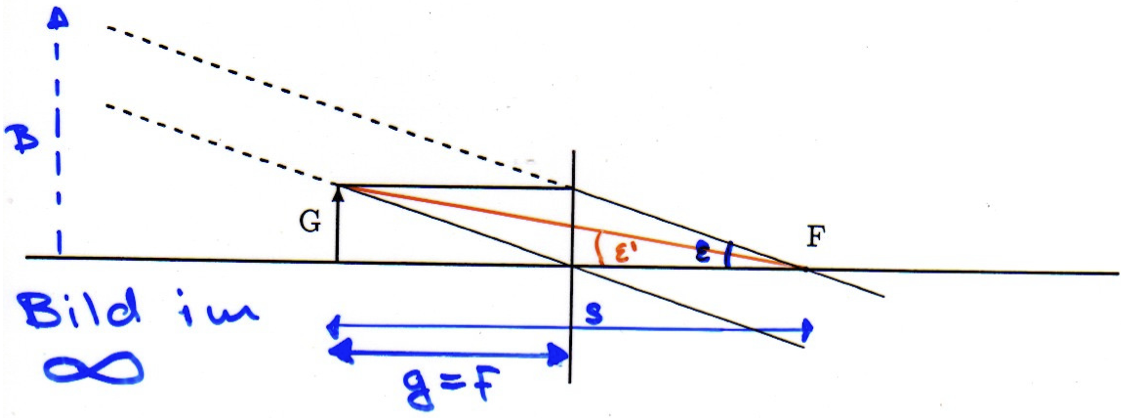
\includegraphics[width=7cm]{./bilder/lupe.png}} &
  \parbox{11cm}{
    Erzeugt virtuelles, vergrössertes \& aufrechtes Bild \\
    \\
    $V \;$ Vergr"osserung \qquad $s \;$ deutliche Sehweite (Auge: 25cm)\\
    \qquad $\varepsilon \;$ Sehwinkel mit \qquad $\varepsilon_0 \;$ Sehwinkel
    ohne Lupe \\
    \\
    $V=\dfrac{s}{f}=\dfrac{\tan(\varepsilon)}{\tan(\varepsilon_0)}\Rightarrow\dfrac{s}{g}>
    V_{\text{normal}}$ }
\end{tabular}
\subsubsection{Projektor \kuchling{377}}
\begin{tabular}{ll}
\parbox{6cm}{
  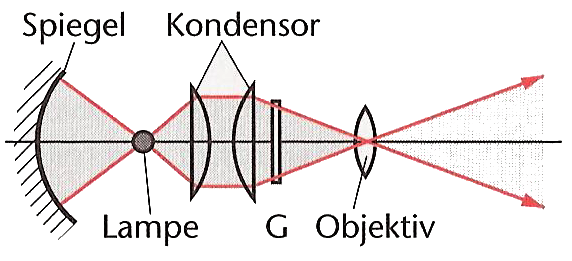
\includegraphics[width=6cm]{./bilder/projektor.png}} &
\parbox{12cm}{
  Erzeugt reelles, vergrössertes \& umgekehrtes Bild \\
  \\
  $\beta \;$ Abbildungsmasstab \\
  $\beta = \dfrac{b}{g} = \dfrac{b}{f}-1$}
\end{tabular}

\subsubsection{Mikroprojektor} 
Erzeugt reelles Bild auf Schirm mit $V=\dfrac{B}{G}=\dfrac{b}{g}$\\

\subsubsection{Mikroskop \kuchling{382} \stoecker{345}}
\begin{tabular}{ll}
  \parbox{8cm}{
    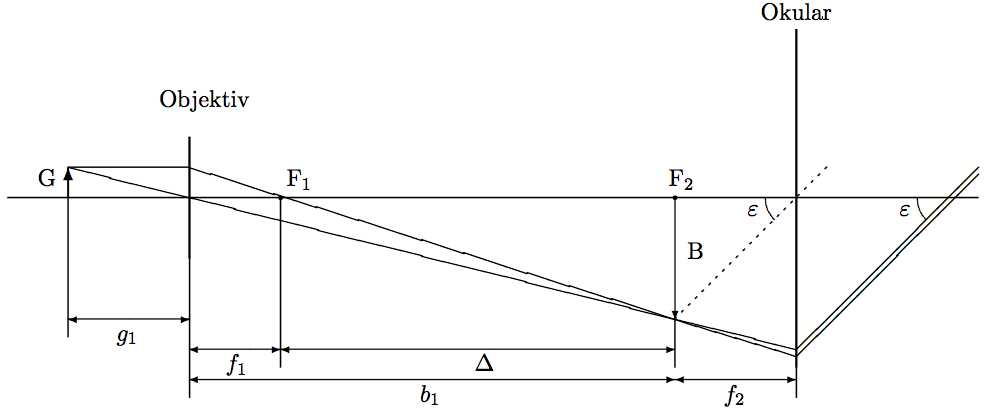
\includegraphics[width=8cm]{./bilder/mikroskop.png}} &
  \parbox{10cm}{
    Erzeugt reelles, vergrössertes \& umgekehrtes Bild. \\
    \\
    $V_1 = \frac{\Delta}{f_1} \;$ Vergrösserung des Objektivs\\
    $V_2 = \frac{s}{f_2} \;$ Vergrösserung des Okulars \\
    \\
    $\Delta = \overline{f_1\,f_2} \;$ Tubuslänge \\
    $V=V_1\,V_2= \dfrac{f_1}{f_2} = \dfrac{\Delta}{f_1} \dfrac{s}{f_2} =
    \dfrac{B}{G} \, \dfrac{s}{f_2}$ }
\end{tabular}

\subsubsection{Keplersches (Astronomisches) Fernrohr \kuchling{383} \stoecker{347}}
\begin{tabular}{ll}
  \parbox{11cm}{
    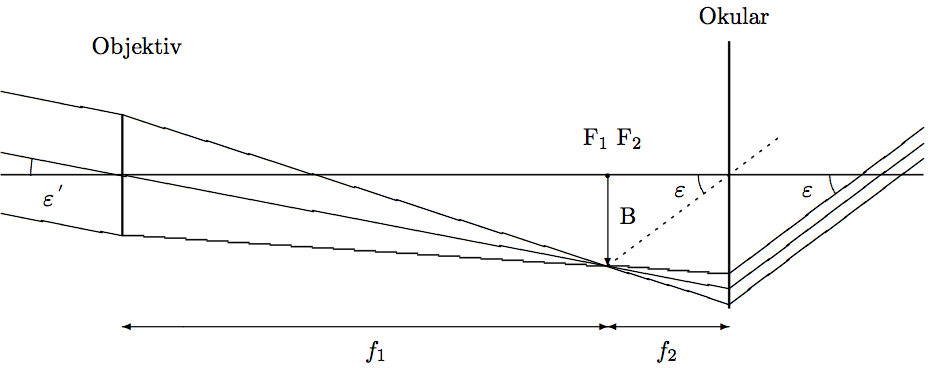
\includegraphics[width=10cm]{./bilder/astron.png}} &
  \parbox{7cm}{
    Erzeugt reelles, vergrössertes \& umgekehrtes Bild. Dies ist ein Spezialfall
    des Mikroskops, wo die \textbf{Gegenstandsweite} auf \textbf{unendlich} ($g \rightarrow \infty$) eingestellt ist. \\
    \\
    $D$ Durchmesser Objektiv \\
    $V$ Vergrösserung\\
    $a$ Abstand Okular-Austrittspupille\\
    $l$ Abstand Objektiv-Okular\\
    $d$ Grösse Austrittspup.\\
    $L$ Lichtstärke }
\end{tabular} \\
$V = \dfrac{\tan(\varepsilon)}{\tan(\varepsilon')} = \dfrac{B/f_2}{B/f_1} =
\dfrac{f_1}{f_2} = \dfrac{D}{d} = \dfrac{f_1+f_2}{a}$ \qquad $l = f_1+f_2$
\qquad $\dfrac{1}{f_1+f_2} + \dfrac{1}{a} = \dfrac{1}{f_2}$ \qquad
$a = \frac{l}{V} $ \qquad $d = \frac{D}{V}$ \qquad $L = d^2 = \left( \frac{D}{V}
\right)^2$

\subsubsection{Diverse \kuchling{384} \stoecker{347}}
\begin{tabular}{ll}
  Terrestr. Fernr. & 
  $V=\left|\dfrac{f_1}{f_2}\right|$ \qquad L"ange: $l=f-|f_2|$ (ent. mit
  Umkehrlinse (ZF), Prismen oder Streul. zur Umkehrung) \\
  Spiegelteleskope &
  Reflexion$\leftrightarrow$Brechung (weniger Lichtv.), k. Dispersion (k. chrom.
  Abberation), Verzug durch Masse  \\
\end{tabular}

\subsection{Konstruktion des Strahlengangs}
\begin{center}
  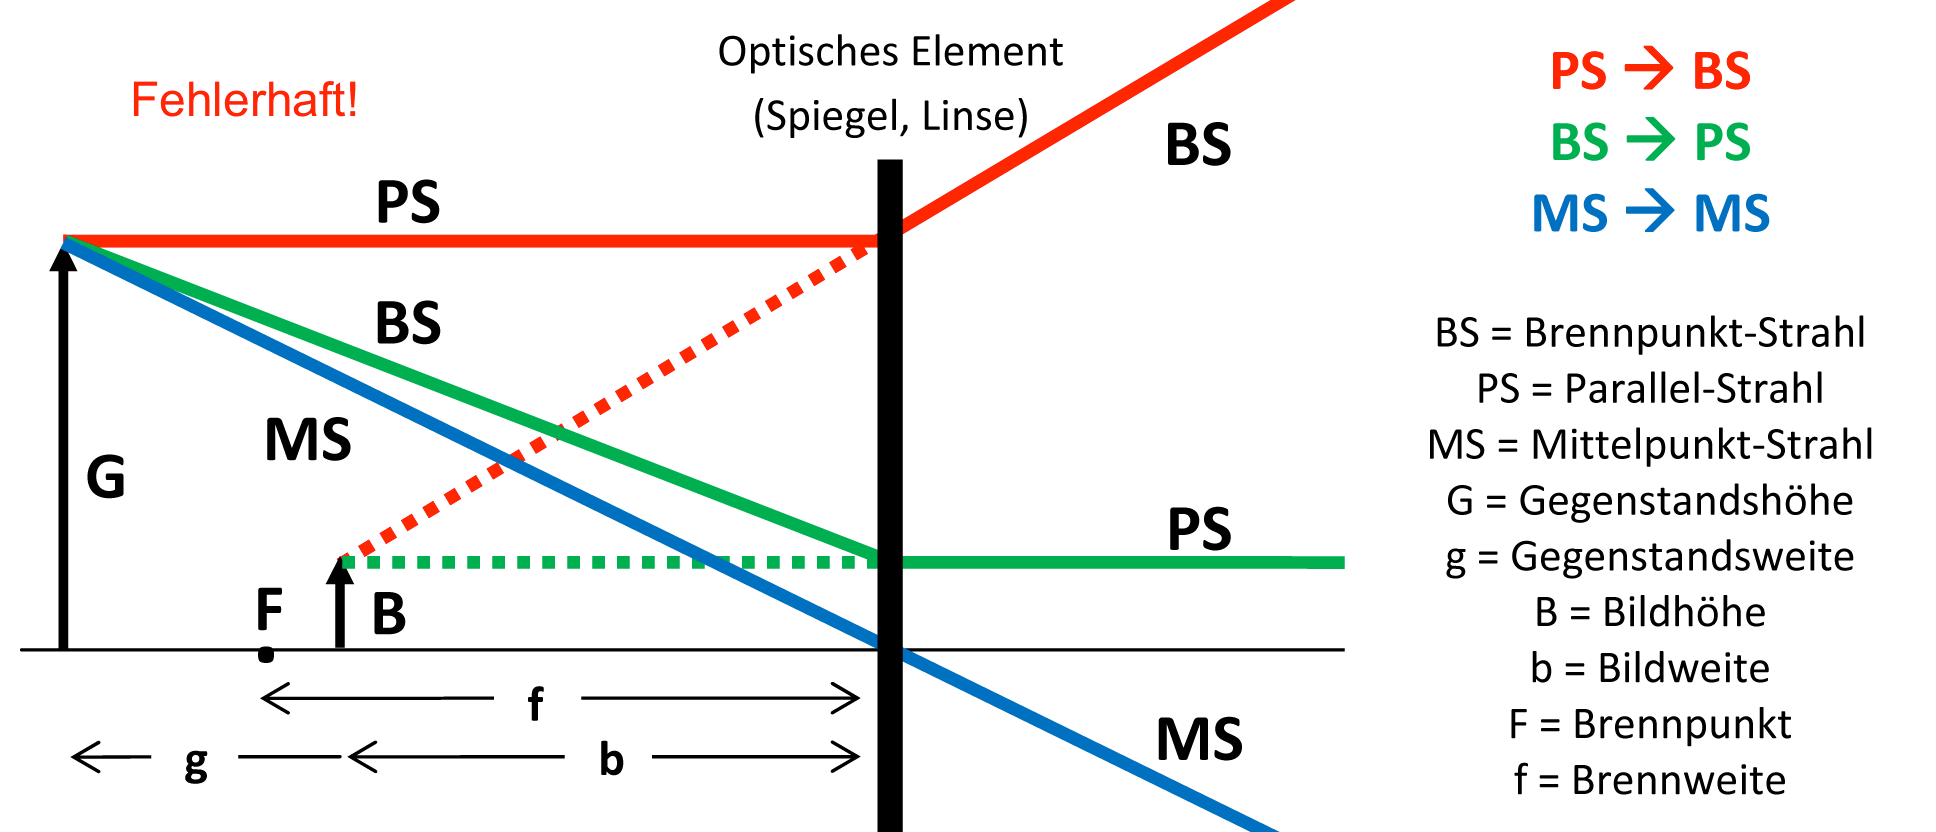
\includegraphics[width=11cm]{./bilder/strahlengang.png}
\end{center}

\section{Schwingungen \kuchling{192} \stoecker{235}}
\subsection{Ungedämpfte Schwingungen}
\renewcommand{\arraystretch}{2}
\begin{tabular}{|p{4cm}|p{8cm}|p{6cm}|}
	\hline
	\begin{minipage}[]{4cm}
    	Harmonische Schwingung\\
    	\kuchling{193} \stoecker{236}\\
    \end{minipage} &
	\begin{minipage}[]{8cm}
 		$y=A\,\sin(\omega t+ \varphi)  \qquad \omega=\dfrac{2\pi}{T}=2\pi f$\\ \\
		$\ddot{y}+\omega^2y=0 \qquad v(t)=\dot{y} \qquad a(t)=\ddot{y}$
    \end{minipage} &
	\begin{minipage}[]{6cm}
        \vspace{0.2cm}
 		$A$ = Amplitude $[1]$\\
 		$\omega$ = Kreisfrequenz $[\frac{1}{s}]$\\
 		$v(t)$ = Geschwindigkeit $[\frac{m}{s}]$\\
 		$a(t)$ = Beschleunigung $[\frac{m}{s^2}]$ 
     \end{minipage}\\
    \begin{minipage}[]{4cm} 
        	Trägheitskraft/Moment
    \end{minipage}&
    \begin{minipage}[]{8cm}
        	Trans. : $F_T(y) = m \cdot \ddot{y} \qquad$
        	Rot.: $M_T(\varphi) = J \cdot \ddot{\varphi}$
    \end{minipage} &\\
	\hline
	\begin{minipage}[]{4cm}
    	Schwingungsenergie\\
    	\kuchling{203} \stoecker{240}\\
    \end{minipage} &
	\begin{minipage}[]{8cm}
    \vspace{0.2cm}
	$E=E_{\text{pot}}+E_{\text{kin}}=\dfrac{c\,y^2}{2}+\dfrac{m\,v^2}{2}= \dfrac{c}{2}\cdot A$\\
	\\ $\dfrac{m\,\omega^2A^2}{2}(\sin(\omega t+\varphi)^2+\cos(\omega
	t+\varphi)^2)=\dfrac{m\,\omega^2\,A^2}{2}$\\
	\end{minipage} &
	\begin{minipage}[]{6cm}
		$E$ = Energie $[J]\\$
		$v=\dot y$ = Geschwindigkeit $[\frac{m}{s}]$\\
		$m$ = Masse $[kg]$\\	
    \end{minipage}\\
	\hline		
	\begin{minipage}[]{4cm}
    	Federpendel\\
    	\kuchling{198} \stoecker{238}\\
    \end{minipage} &
	\begin{minipage}[]{8cm}
    	\underline{ohne Federmasse:}\\
		$m\ddot{y}+c\,y=0 \qquad \omega_0=\sqrt{\dfrac{c}{m}} = \sqrt{\dfrac{c_1 +
		c_2}{m_1 + m_2}}$ \\ $T=2\pi \sqrt{\dfrac{m}{c}}$\\ \\
		rücktr. Kraft: $F=-cy=m\,\ddot{y} = F_T$ \\ \\
		\underline{mit Federmasse:}\\
		$\omega_0=\sqrt{\dfrac{c}{m+\frac{m_F}{3}}} \qquad
		T=2\pi\sqrt{\dfrac{m+\frac{m_F}{3}}{c}}$\\ 
		\end{minipage} &
	\begin{minipage}[]{6cm}
		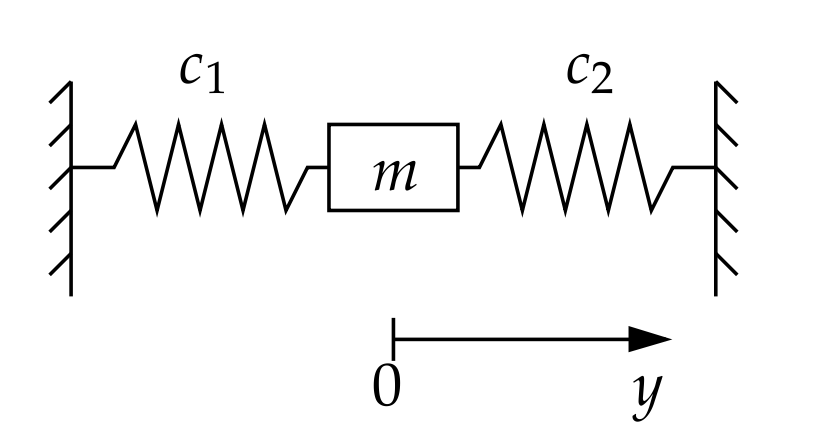
\includegraphics[width=3.5cm]{./bilder/Federpendel_masselos.png}\\ \\
		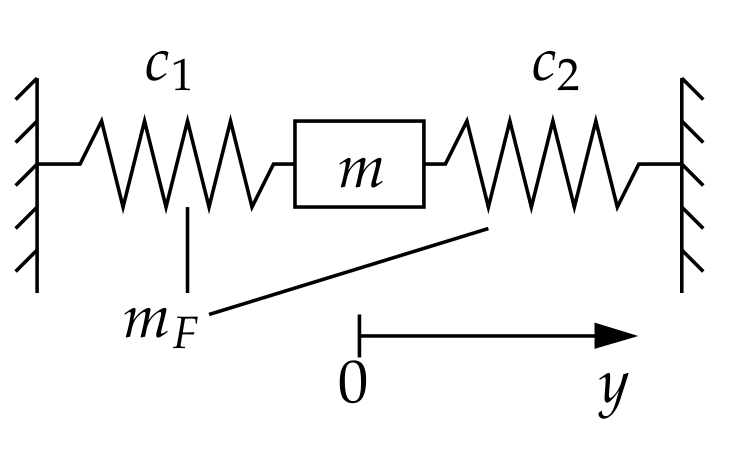
\includegraphics[width=3.5cm]{./bilder/Federpendel_masse.png}	\\		
    \end{minipage}\\
	\hline
	\begin{minipage}[]{4cm}
    	Drehpendel\\
    	\kuchling{199} \stoecker{245}\\
    \end{minipage} &
	\begin{minipage}[]{8cm}
	$J\ddot{\varphi}+c_{_D}\varphi=0 \qquad \omega_0=\sqrt{\dfrac{c_{_D}}{J}} \qquad
	T=2\pi\sqrt{\dfrac{J}{c_{_D}}}$\\ \\
	rücktr. Drehm.:	$M=-c_{_D}\,\varphi=J\,\ddot{\varphi}$ (Bewegung)\\
	\end{minipage} &
	\begin{minipage}[]{6cm}
    	\vspace{0.1cm}
		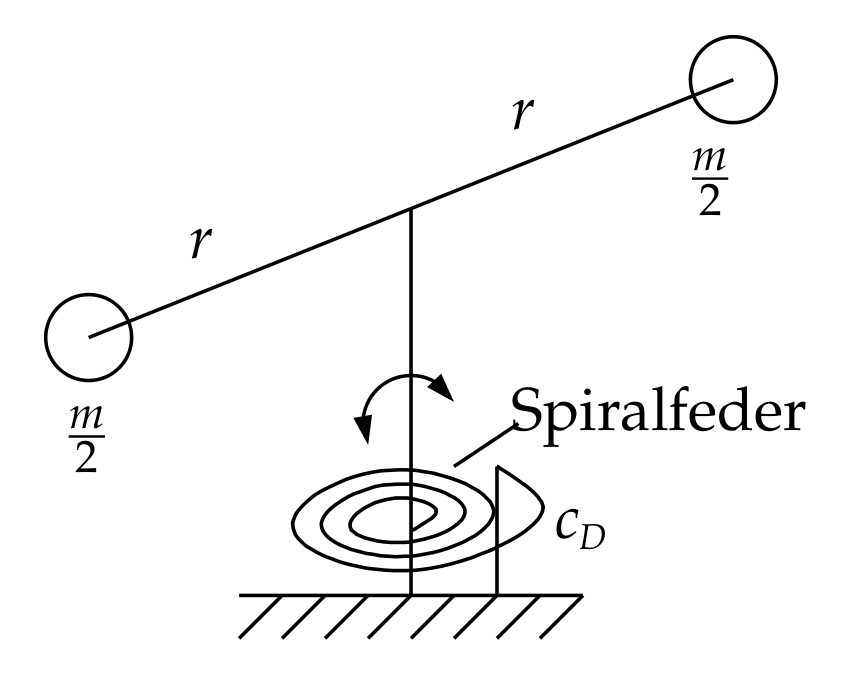
\includegraphics[width=3.5cm]{./bilder/Drehpendel.png}	
    \end{minipage}\\
	\hline
	\begin{minipage}[]{4cm}
    	Fadenpendel,\\
    	Mathematisches Pendel\\
    	\kuchling{200} \stoecker{240}\\
    \end{minipage} &
	\begin{minipage}[]{8cm}
	$l\ddot{\varphi}+g\sin(\varphi)=0\quad\xrightarrow{\text{lin.} (\varphi \ll 1)}\quad
	l\ddot{\varphi}+g\varphi=0$\\ \\
	$\omega_0=\sqrt{\dfrac{g}{l}} \qquad T=2\pi\sqrt{\dfrac{l}{g}} \qquad
	v=l\dot{\varphi} \qquad a=l\ddot{\varphi}$\\
	\end{minipage} &
	\begin{minipage}[]{6cm}
    	\vspace{0.1cm}
		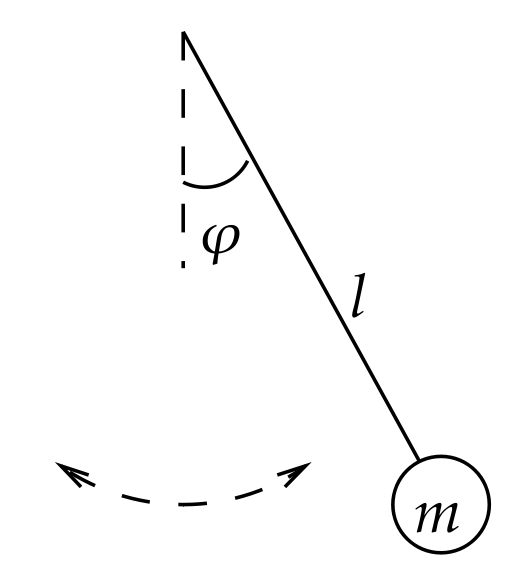
\includegraphics[width=2cm]{./bilder/mathe_pendel.png}	
    \end{minipage}\\
	\hline
	\begin{minipage}[]{4cm}
    	Physisches Pendel\\
    	\kuchling{201} \stoecker{243}\\ \\ \\
    	Massenträgheitsmomente\\
    	\kuchling{131} \stoecker{103}\\
    \end{minipage} &
	\begin{minipage}[]{8cm}
    \vspace{0.2cm}
	$J_A\ddot{\varphi}+m\,g\,a\sin(\varphi)=0$ $\xrightarrow{\text{lin.}}$ $
	J_A\ddot{\varphi}+m\,g\,a\,\varphi=0$\\ \\
	$\omega_0 = \sqrt{\dfrac{m\,g\,a}{J_A}}=\sqrt{\dfrac{g}{l^{*}}} \qquad
	T=2\pi\sqrt{\dfrac{J_A}{m\,g\,a}}=2\pi\sqrt{\dfrac{l^*}{g}}$\\ \\
	$l^{*}=\dfrac{J_A}{m\,a}=\dfrac{J_M}{m\,x} = \dfrac{J_{S}}{m\cdot a}+a$\\ 
	bei mehreren Elementen: \parbox{3cm}{
			$J_A = \sum J_{A_i}$\\
				 $m = \sum m_i$}\\ \\
	$J_A=J_S+m\,a^2 \qquad J_M=J_S+m\,x^2$\\ \\
	\textbf{Perkussionszentrum}\\
	Trifft ein Schlag den Schwingungsmittelpunkt $M$ wirken keine Kräfte auf den
	Punkt $A$ \& umgekehrt\\
	\textbf{Minimale Schwingungsdauer}\\
	$l_{min}^* = 2\sqrt{\dfrac{J_S}{m}}$ wenn $a=x=a_{min}$
	\end{minipage} &
	\begin{minipage}[]{6cm}
		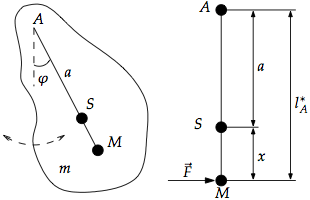
\includegraphics[width=6cm]{./bilder/physpendel.png}\\	
		\vspace{0.2cm}
		$\l^*$ = reduzierte Pendellänge\\
		$\l_A^* = l_M^*$
    \end{minipage}\\
	\hline
	\begin{minipage}[]{4cm}
    	Schwerpunkt berechnen\\
    	\kuchling{66} \stoecker{84}\\
    \end{minipage} &
	\begin{minipage}[]{8cm}
		$\vec{R}=\dfrac{\sum_i \vec{r_i} \Delta m_i}{m} \qquad m=\sum_i \Delta m_i$
	\end{minipage} &
	\begin{minipage}[]{6cm}
    	\vspace{0.2cm}
		$\vec{R}$ = Ortsvektor des Schwerpunkts\\
		$\vec{r_i}$ = Koordinate des $i$-ten Elements\\
		$\Delta m_i$ = Masse des $i$-ten Elements
    \end{minipage}\\
	\hline	
\end{tabular}
\renewcommand{\arraystretch}{1}

\subsection{Gedämpfte Schwingungen}
\renewcommand{\arraystretch}{2}
\begin{tabular}{|p{4cm}|p{8cm}|p{6cm}|}
	\hline
	\begin{minipage}[]{4cm}
    	Konstante Reibung\\
    	\kuchling{205} \stoecker{249}\\
    \end{minipage} &
	\begin{minipage}[]{8cm}
    	\vspace{0.2cm}
		$m\ddot{y}+cy+F_R=0 \qquad F_R=\mu\,F_N \qquad \Delta A=4\dfrac{F_R}{c} $\\
		Masse bleibt stehen, wenn $c\cdot A_n < F_R$
	\end{minipage} &
	\begin{minipage}[]{6cm}
        \vspace{0.2cm}
 		$\Delta A$ = Abnahme von $A$ pro Periode $[m]$\\
 		$F_R$ = Reibkraft $[N]$\\
 		$c$ = Federkonstante $[\frac{N}{m}]$\\ 
    \end{minipage}\\
	\hline
	\begin{minipage}[]{4cm}
    	Geschwindigkeitsprop. Dämpfung\\
    	\kuchling{205} \stoecker{250}\\
    \end{minipage} &
	\begin{minipage}[]{8cm}
	    \vspace{0.2cm}
	    \underline{$D<1$: Schwingfall}\\
		$m\,\ddot{y}+b\,\dot{y}+c\,y=\ddot{y}+\underbrace{\dfrac{b}{m}}_{2\delta}
		\cdot\dot{y}+\underbrace{\dfrac{c}{m}}_{\omega_0^{\,2}}\cdot y=0$\\
		$\qquad F_d=-b\dot y$\\ \\
		Ansatz abklingende Schwingung: \\
		$y(t)=A e^{-\delta t}\sin(\omega_d t+\varphi_0)$\\ \\
		$\delta=\dfrac{b}{2m}$\\
		$\omega_0=\sqrt{\dfrac{c}{m}}$ \\ 
		$\omega_d =	\omega_0 \sqrt{1-D^2} = \sqrt{\dfrac{c}{m}-\delta^2}=
		\sqrt{\omega_0^2 - \delta^2}$\\
		\\
		$\omega_r=\omega_0\sqrt{1-2\cdot D^2}$\\ \\
		$D=\dfrac{\delta}{\omega_0}=\dfrac{\frac{\Lambda}{2\pi}}{\sqrt{1+\left(\frac{\Lambda}{2\pi}\right)^2}} \approx \dfrac{\Lambda}{2\pi}$ (für kleine $D$)\\
		$\Lambda=\delta T=\dfrac{2\pi D}{\sqrt{1-D^2}}=\ln{\dfrac{\hat
		A_n}{\hat A_{n+1}}}\qquad\dfrac{\hat A_n}{\hat A_{n+1}}=e^{\delta T}$\\ 
		$\dfrac{A_{n+1}}{A_n} = \sqrt[\mathlarger{\mathlarger{k}}]{\dfrac{A_{n+k}}{A_n}}$\\ \\
		$\dfrac{E_t}{E_{t+\Delta t}}=\dfrac{A_t^2}{A_{t+\Delta t}^2} \qquad
		\dfrac{A_t}{A_{t+\Delta t}}= e^{\delta \Delta t} $\\ \\ \\
		\underline{$D>1$: Kriechfall (keine Schwingung mehr)}\\ \\
		$y(t)=b_1 e^{\lambda_1 t}+b_2e^{\lambda_2 t}$\\ \\
		$\lambda_1=-\omega_0(D+\sqrt{D^2-1})\quad\lambda_2=-\omega_0(D-\sqrt{D^2-1})$\\ \\
		\underline{$D=1$: Aperiodischer Grenzfall ($\delta = \omega_0$)}\\ \\
		$y=(b_1+b_2 t)\,e^{-\delta t} \qquad
		\omega_0^2=\dfrac{c}{m}=\dfrac{b^2}{4m^2}=\delta^2$\\
	\end{minipage} &
	\begin{minipage}[]{6cm}
 		$m$ = Mitschwingende Masse $[kg]$\\
 		$b$ = Dämpfungskonstante $[\frac{kg}{s}]$\\
 		$c$ = Federkonstante $[\frac{N}{m}]$\\
 		$F_d$ = Geschwindigkeits-proportionale Dämpfungskraft\\ \\
 		$\omega_0$ = Eigen-Kreisfr. $[\frac{1}{s}]$\\
 		$\omega_d$ = gedämpfte Kreisfr. $[\frac{1}{s}]$\\
 		$\omega_r$ = Resonanzkreisfrequenz $[\frac{1}{s}]$\\ \\ 				
 		$T$ = Periodendauer $[s]$\\
 		$A$ = Amplitude $[1]$\\
 		$\varphi_0$ = Phasenwinkel $[rad]$ \\ 		
 		$E$ = Energie $[J]$\\ \\
 		$\delta$ = Abklingkostante $[1/s]$\\
 		$D$ = Dämpfungsgrad $[1]$\\
		
 		$\Lambda$ = logartihmisches Dekrement $[1]$\\ \\
 		$\hat A_n$ = $A_{max}$ zu Zeitpunkt $t_n$ $[1]$\\
  		$\hat A_{n+1}$ = $A_{max}$ zu Zeitpunkt $t_n+T$ $[1]$\\
  		$E_t$ = $E$ zu Zeitpunkt $t$ $[J]$\\
  		$E_{t+\Delta t}$ = $E$ zu Zeitpunkt $t+\Delta t$ $[J]$\\
  		$A_t$ = $A$ zu Zeitpunkt $t$ $[1]$\\
  		$A_{t+\Delta t}$ = $A$ zu Zeitpunkt $t+\Delta t$ $[1]$\\	\\ \\ \\ \\ \\ \\
  		$b_1$ \& $b_2$ durch Anfangsbedingungen			
    \end{minipage}\\
	\hline	
\end{tabular}

\begin{multicols}{2}
\subsection{Diverse Formeln}
\begin{tabular}{|l|l||l|}
	\hline
	\textbf{Translation}	& \textbf{Rotation} & \textbf{Diverses}\\
	\hline
	\hline
	$x=$ Weg & $\varphi=$ Weg& 
	$F=m\cdot a$\\
	\hline
	$v=\dot{x}$ & $\omega=\dot{\varphi}$&
	$F=m\cdot\alpha\cdot r$\\
	\hline
	$a=\dot{v}=\ddot{x}$ & $\alpha=\dot{\omega}=\ddot{\varphi}$&
	$M=J\cdot\alpha=J\cdot\ddot{\varphi}$\\
	\hline
\end{tabular}

\subsection{Federn in Serie und Parallel}
\textbf{Parallel:} $c = c_1 + c_2$ \\
\textbf{Serie:} $ \frac{1}{c} = \frac{1}{c_1} + \frac{1}{c_2} \longrightarrow
c = \frac{c_1c_2}{c_1 + c_2}$
\end{multicols}
\newpage

\subsection{Fremderregte Schwingungen \kuchling{213} \stoecker{254}}
Die \textcolor{blue}{Erregungsschwingung} ist jeweils das Störglied der DGL.\\

\begin{tabular}{|l|l|}
\hline
\textbf{Allgemein}

	& \begin{minipage}[]{12cm}
      \renewcommand{\arraystretch}{2}      
		\begin{tabular}{lll}
    	Dimensionslose Frequenz
    		& $\eta=\dfrac{\omega}{\omega_0}$ 
			& $\omega$ = Erregerkreisfrequenz \\
    	Eigenkreisfrequenz
    		& $\omega_0 = \sqrt{\dfrac{c}{\sum m}}$
			& Federn parallel: $\omega_0 =
    		\sqrt{\dfrac{\sum c}{\sum m}}$
		\end{tabular} \\
    \end{minipage} \\
\hline
\hline
\parbox{6cm}{
	\textbf{Kraft- / Federkrafterregung}\\
	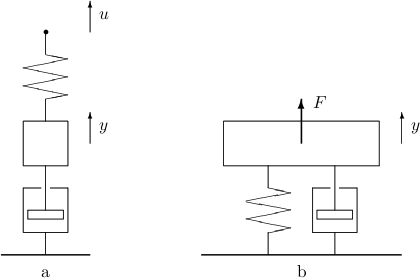
\includegraphics[width=6cm]{./bilder/federkrafterregung.png}}
	& \begin{minipage}[]{12cm}
      \renewcommand{\arraystretch}{2}      
		\begin{tabular}{ll}
    	Differentialgleichung
    		& $m \, \ddot{y} + b \, \dot{y} + c y=$
    		\textcolor{blue}{$c \, u_0 \, \sin(\omega t)$} \\
    	Amplitude
    		&
    		$A=\dfrac{c\,u_0}{m\sqrt{(\omega_0^2-\omega^2)^2+(2D\,\omega_0\,\omega)^2}}$ \\
    	Phase zw. $\omega_0$ \& $\omega$
    		&
    		$\varphi=\arctan\left(\dfrac{2D\,\omega_0\,\omega}{\omega_0^2-\omega^2}\right)$\\ 
    	Resonanzkreisfrequenz
    		& $\omega_r=\omega_0\sqrt{1-2D^2}$\quad $\omega_r<\omega_d<\omega_0$\\
    	Resonanzamplitude
    		& $A_r=\dfrac{u_0}{2D\sqrt{1-D^2}} = \dfrac{c \cdot u_0}{2m\sqrt{(\delta \omega_0)^2 - \delta^4}}$\\
    	Vergrösserungsfunktion
    		&
    		$V=\dfrac{1}{\sqrt{(1-\eta^2)^2+(2D\eta)^2}}=\dfrac{A(\omega)}{u_0}$ \\ 
    	Vergrösserung bei Resonanz
    		&
    		$V_r = \dfrac{1}{\sqrt{1-\eta_r^4}}$ mit $\eta_r = \sqrt{1-2D^2}$\\
    	\multicolumn{2}{l}{\parbox{12cm}{\small
    	Überkritische Dämfpung, wenn $D > \frac{1}{\sqrt2} \Rightarrow$ Auch bei 
    	Resonanz\\
    	bleibt Amplitude stets unter statischer
    	Auslenkung ($V \leq 1$)}}
		\end{tabular}
    \end{minipage} \\
\hline
\parbox{6cm}{
	\textbf{Indirekte Federkrafterregung}\\
	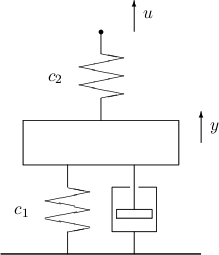
\includegraphics[width=4cm]{./bilder/indirekte-federkrafterregung.png}}
	& \begin{minipage}[]{12cm}
      \renewcommand{\arraystretch}{2}
		\begin{tabular}{ll}
    	Differentialgleichung
    		& $m \, \ddot{y} + b \, \dot{y} + c y=$
    		\textcolor{blue}{$c_2 \, u_0 \, \sin(\omega t)$} \\
    	Amplitude
    		&
    		$A=\dfrac{c_2}{c} 
    		\dfrac{c\,u_0}{m\sqrt{(\omega_0^2-\omega^2)^2+(2D\,\omega_0\,\omega)^2}}$ \\
    	Phase zw. $\omega_0$ \& $\omega$
    		&
    		$\varphi=\arctan\left(\dfrac{2D\,\omega_0\,\omega}{\omega_0^2-\omega^2}\right)$\\ 
    	Resonanzkreisfrequenz
    		& $\omega_r=\omega_0\sqrt{1-2D^2}$\\
    	Resonanzamplitude
    		& $A_r=\dfrac{u_0}{2D\sqrt{1-D^2}}$\\
    	Vergrösserungsfunktion
    		&
    		$V=\dfrac{c_2}{c}\cdot\dfrac{1}{\sqrt{(1-\eta^2)^2+(2D\eta)^2}}$
		\end{tabular}
    \end{minipage} \\
\hline
\parbox{6cm}{
	\textbf{Dämpferregung}\\ \\
	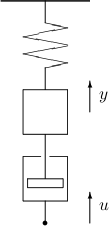
\includegraphics[width=2cm]{./bilder/daempferregung.png}}
	& \begin{minipage}[]{12cm}
      \renewcommand{\arraystretch}{2}
		\begin{tabular}{ll}
    	Differentialgleichung
    		& $m\,\ddot{y}+b\,\dot{y}+c\,y=$
    		\textcolor{blue}{$b\,\omega\,u_0\,\sin(\omega t+\frac{\pi}{2})$} \\
    	Amplitude
    		&
    		$A=\dfrac{b\,\omega\,u_0}{m\sqrt{(\omega_0^2-\omega^2)^2+(2D\,\omega_0\,\omega)^2}}$ \\
    	Phase zw. $\omega_0$ \& $\omega$
    		&
    		$\varphi=\operatorname{arctan}\left(\dfrac{2D\,\omega_0\,\omega}{\omega_0^2-\omega^2}\right)-\dfrac{\pi}{2}$\\ 
    	Resonanzkreisfrequenz
    		& $\omega_r=\omega_0 \quad \rightarrow$\quad max. bei $\eta=1$\\
    	Resonanzamplitude
    		& $A_r=u_0\quad\rightarrow\quad V(1)=1$\\
    	Vergrösserungsfunktion
    		&
    		$V=\dfrac{2 \,D\, \eta}{\sqrt{(1-\eta^2)^2+(2D\eta)^2}}$ 
		\end{tabular}
    \end{minipage} \\
\hline
\end{tabular}
\newpage
\begin{tabular}{|l|l|}
\hline
\parbox{6cm}{
	\textbf{Stützenerregung}\\ \\
	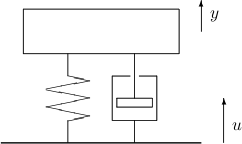
\includegraphics[width=4cm]{./bilder/stuetzenerregung.png}}
	& \begin{minipage}[]{12cm}
      \renewcommand{\arraystretch}{2}
		\begin{tabular}{ll}
    	Differentialgleichung
    		& $m\,\ddot{y}+b\,\dot{y}+c\,y=$
    		\textcolor{blue}{$c\,u_0\,\sin(\omega t) + b\,\omega\,u_0\,\cos(\omega t)$}
    		\\ & $m\, \ddot{q} + b\,\dot{q} + c\,q =$
    		\textcolor{blue}{$m\,\omega^2\,u_0\,\sin(\omega t)$} \\
    	Amplitude
    		&
    		$A=\dfrac{\omega^2\,u_0}{\sqrt{(\omega_0^2-\omega^2)^2+(2D\,\omega_0\,\omega)^2}}$ \\
    	Phase zw. $\omega_0$ \& $\omega$
    		&
    		$\varphi=\arctan\left(\dfrac{2D\,\omega_0\,\omega}{\omega_0^2-\omega^2}\right)-\pi$\\ 
    	Resonanzkreisfrequenz
    		& $\omega_r=\dfrac{\omega_0}{\sqrt{1-2D^2}}$\\
    	Resonanzamplitude
    		& $A_r=\dfrac{u_0}{2D\sqrt{1-D^2}}$\\
    	Vergrösserungsfunktion
    		& $V=\dfrac{\eta^2}{\sqrt{(1-\eta^2)^2+(2D\eta)^2}}$ 
		\end{tabular}
    \end{minipage} \\
\hline
\parbox{6cm}{
	\textbf{Unwuchterregung}\\ \\
	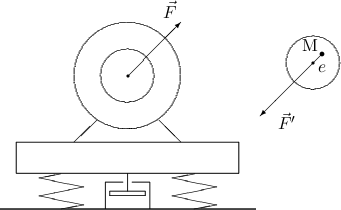
\includegraphics[width=6cm]{./bilder/unwuchterregung.png}\\ \\
	$m_R$ Rotormasse (bewegt)\\
	$e$ Exzentrizit"at (Distanz Achse$\leftrightarrow$SP) \\
	$F_0$ Kraft auf Fundament ohne Federung\\
	$F_{B0}$ verringerte Kraft}
	& \begin{minipage}[]{12cm}
      \renewcommand{\arraystretch}{2}
		\begin{tabular}{ll}
        $F(t)=F_0\cdot\sin(\omega t)$
        	& $F_0=m\cdot a_r=m\cdot\dfrac{v^2}{r}=m\cdot r\cdot \omega^2=m_R\cdot e \cdot \omega^2$ \\
    	Differentialgleichung
    		& $m\,\ddot{y}+b\,\dot{y}+c\,y=$
    		\textcolor{blue}{$m_R\,e\,\omega^2\,\sin(\omega t)$} \\
    	Amplitude
    		&
    		$A=\dfrac{m_R\,e\,\omega^2}{m\sqrt{(\omega_0^2-\omega^2)^2+(2D\,\omega_0\,\omega)^2}}$ \\
    	Phase zw. $\omega_0$ \& $\omega$
    		&
    		$\varphi=\operatorname{arctan}\left(\dfrac{2D\,\omega_0\,\omega}{\omega_0^2-\omega}\right)$\\ 
    	Resonanzkreisfrequenz
    		& $\omega_r=\dfrac{\omega_0}{\sqrt{1-2D^2}}$\\
    	Resonanzamplitude
    		& $A_r=\dfrac{m_R}{m}\dfrac{e}{2D\sqrt{1-D^2}}$\\
    	Kraftamplitude \textbf{ohne} Fed.
    		& $F_0 = m_R\,e\,\omega^2 \sin(\omega t)$\\
		Kraftamplitude \textbf{mit} Fed.
    		&
    		$F_{B0}=\dfrac{m_R\,e\,\omega^2\,\sqrt{1+4D^2\eta^2}}{\sqrt{(1-\eta^2)^2+4D^2\eta^2}}=F(\eta)$ \\ 
    	Verhältnis
    		&$\dfrac{F_{B0}}{F_0}=\sqrt{\dfrac{1+4D^2\eta^2}{(1-\eta^2)^2+4D^2\eta^2}}$ \\ 
		\end{tabular}
    \end{minipage} \\
\hline
\end{tabular}
\renewcommand{\arraystretch}{1}

\newpage

\subsection{Schwingkreise}
\subsubsection{Serienschwingkreis \kuchling{530} \stoecker{253}}
\renewcommand{\arraystretch}{2}
\begin{tabular}{|p{4cm}|p{14cm}|}
\hline
Diffgl: &
\begin{minipage}[]{14cm}
\vspace{0.2cm}
$L\ddot{I}+R_S\dot{I}+\dfrac{1}{C}\,I=\omega\,U_0\,\sin(\omega t +
\dfrac{\pi}{2})$ \qquad $I=I_0\,e^{-\delta t}\,\sin(\omega_d t+\varphi)$\\
\end{minipage}\\
\hline
Amplitude: &
\begin{minipage}[]{14cm}
\vspace{0.2cm}
$I_0=\dfrac{\omega\,U_0}{L\sqrt{(\omega_0^{\,2}-\omega^2)^2+(2D\,\omega_0\,\omega)^2}}$\\
\end{minipage}\\
\hline
Phase: &
\begin{minipage}[]{14cm}
\vspace{0.2cm}
$\varphi=\arctan{\dfrac{2D\,\omega_0\,\omega}{\omega_0^{\,2}-\omega^2}}-\dfrac{\pi}{2}$\\
\end{minipage}\\
\hline
Resonanzfrequenz: &
\begin{minipage}[]{14cm}
\vspace{0.2cm}
$\omega_r=\omega_0=\dfrac{1}{\sqrt{LC}}$ \qquad
$\omega_d=\omega_0\sqrt{1-D^2}=\dfrac{1}{\sqrt{LC}}\,\sqrt{1-\dfrac{R^2C}{4L}}$\\
\end{minipage}\\
\hline
Resonanzamplitude: &
\begin{minipage}[]{14cm}
\vspace{0.2cm}
$I_{0_r}=\dfrac{U_0}{R_S}$\\
\end{minipage}\\
\hline
Vergr"osserungsfunktion: &
\begin{minipage}[]{14cm}
\vspace{0.2cm}
$V(\eta)=\dfrac{\eta^2}{\sqrt{(1-\eta^2)^2+(2D\,\eta)^2}}$\qquad Max:
$V_m=\dfrac{1}{2D\sqrt{1-D^2}}$\\
\end{minipage}\\
\hline
Phasenverschiebung: &
\begin{minipage}[]{14cm}
\vspace{0.2cm}
$\varphi_U=\arctan\left(\dfrac{2D\,\eta}{1-\eta^2}\right)-\pi$\\
\end{minipage}\\
\hline
D"ampfungsgrad: &
\begin{minipage}[]{14cm}
\vspace{0.2cm}
$D=\dfrac{R_S}{2}\sqrt{\dfrac{C}{L}}$\\
\end{minipage}\\
\hline
Abklingkonst. : &
\begin{minipage}[]{14cm}
\vspace{0.2cm}
$\delta=\dfrac{R_S}{2L}$\\
\end{minipage}\\
\hline
\end{tabular}

\subsubsection{Parallelschwingkreis}
\begin{tabular}{|p{4cm}|p{14cm}|}
\hline
Diffgl: &
\begin{minipage}[]{14cm}
\vspace{0.2cm}
$C\ddot{U}+\dfrac{1}{R_P}\dot{U}+\dfrac{1}{L}U=\omega\,I_0\,\sin(\omega
t+\dfrac{\pi}{2})$\\
\end{minipage}\\
\hline
Amplitude: &
\begin{minipage}[]{14cm}
\vspace{0.2cm}
$U_0=\dfrac{\omega\,I_0}{C\sqrt{(\omega_0^{\,2}-\omega^2)^2+(2D\,\omega_0\,\omega)^2}}$\\
\end{minipage}\\
\hline
Phase: &
\begin{minipage}[]{14cm}
\vspace{0.2cm}
$\varphi=\arctan{\dfrac{2D\,\omega_0\,\omega}{\omega_0^{\,2}-\omega^2}}-\dfrac{\pi}{2}$\\
\end{minipage}\\
\hline
Resonanzfrequenz: &
\begin{minipage}[]{14cm}
\vspace{0.2cm}
$\omega_r=\omega_0=\dfrac{1}{\sqrt{LC}}$\\
\end{minipage}\\
\hline
Resonanzamplitude: &
\begin{minipage}[]{14cm}
\vspace{0.2cm}
$U_{0_r}=I_0\cdot R_P=\dfrac{\omega^2\,L^2}{R_S}$\\
\end{minipage}\\
\hline
Vergr"osserungsfunktion: &
\begin{minipage}[]{14cm}
\vspace{0.2cm}
$V(\eta)=\dfrac{1}{\sqrt{(1-\eta^2)^2+(2D\,\eta)^2}}$\qquad Max:
$V_m=\dfrac{1}{2D\sqrt{1-D^2}}$\\
\end{minipage}\\
\hline
Phasenverschiebung: &
\begin{minipage}[]{14cm}
\vspace{0.2cm}
$\varphi_I=\arctan\left(\dfrac{2D\,\eta}{1-\eta^2}\right)$\\
\end{minipage}\\
\hline
D"ampfungsgrad: &
\begin{minipage}[]{14cm}
\vspace{0.2cm}
$D=\dfrac{1}{2\,R_P}\sqrt{\dfrac{L}{C}}$\\
\end{minipage}\\
\hline
\end{tabular}
\renewcommand{\arraystretch}{1}

\subsubsection{G"ute}
$Q=2\pi\dfrac{E(t)}{E(t)-E(t+T)}=\dfrac{1}{2D}=V_m=\dfrac{\omega_0}{\Delta \omega}$\quad wobei \quad $E=\dfrac{C\,U^2}{2}+\dfrac{L\,I^2}{2}=\dfrac{L\,I_0^{\,2}}{2}=\dfrac{L\,\omega_0^{\,2}\,C^2\,U_0^{\,2}}{2}=\dfrac{C\,U_0^{\,2}}{2}$

\section{Wellen / Akustik \kuchling{229} \stoecker{265}}
\subsection{Definitionen räumlicher Elemtarwellen}
\begin{tabular}[]{|p{9cm}|p{9cm}|}
	\hline
	\begin{minipage}{9cm}
		\textbf{Wellengleichung:}\\
			$\ddot{\xi} = u^2 \cdot \xi''(x)$
	\end{minipage} &
	\begin{minipage}[]{9cm}
			$\ddot{\xi}$ = Zweite Ableitung nach der Zeit\\
			$\xi''$ = Zweite Ableitung nach dem Ort
	\end{minipage}\\
	\begin{minipage}[]{9cm}
    	\textbf{Ebene harmonische Welle:}\\
 		$\xi(\vec{r},t)=\xi_0 \sin(\omega t -k\vec{r}+\varphi)$\\ \\		   	
 		$\xi(\vec{r},t)=\xi_0 e^{-j(\omega t-k\vec{r})}$\\ \\ 
 		\textbf{Harmonische Kugelwelle:}\\
 		$\xi(\vec{r},t)=\dfrac{\xi_0}{|\vec{r}|} \sin(\omega
 		t-k|\vec{r}|+\varphi)$\\\\
 		$\xi(\vec{r},t)=\dfrac{\xi_0}{|\vec{r}|} e^{-j(\omega t-k|\vec{r}|)}$\\ 		
    \end{minipage} &
	\begin{minipage}[]{9cm}
    	\vspace{0.2cm}    
    	$\xi({\vec{r},t})$ = Auslenkung am Ort $\vec{r}$ zur Zeit $t$\\
		$\xi_0$ = Amplitude $[1]$\\
		$k$ = Wellenzahl $[\frac{1}{m}]$\\
		$\vec{r}$ = Ortsvektor $[m]$\\
		$\omega$ = Kreisfrequenz $[\frac{1}{s}]$\\
		$\varphi$ = Phasenverschiebung $[rad]$\\    
		$\lambda$ = Wellenlänge $[m]$\\
		$u$ = Wellengeschwindigkeit $[\frac{m}{s}]$\\
		$f$ = Frequenz $[Hz]$\\
		$T$ = Periodendauer $[s]$\\
    \end{minipage} \\
	\hline
\end{tabular}

\subsection{Wichtige Beziehungen}
$\boxed{k=\dfrac{\omega}{u}=\dfrac{2\pi}{\lambda}}$\quad
$\boxed{u=\dfrac{\omega}{k} = \lambda \cdot f}$ \quad
$\boxed{\lambda=\dfrac{2\pi}{k}=\dfrac{u}{f}}$ \quad
$\boxed{\omega=2\pi f=\dfrac{2\pi}{T}}$ \quad
$\boxed{f=\dfrac{\omega}{2\pi}=\dfrac{u}{\lambda}=\dfrac{1}{T}}$ \quad
$\boxed{T=\dfrac{1}{f}=\dfrac{2\pi}{\omega}}$ \quad
$\boxed{\varphi=\omega t-k|\vec{r}|}$

\subsection{Wellengeschwindigkeit \kuchling{233} \stoecker{267}}
\renewcommand{\arraystretch}{1.5}
\begin{tabular}{| p{6cm} | p{6cm} | p{6cm} |}
\hline
\textbf{Elastisch}e L"angs-/ Longitudinalwelle & \textbf{Elastisch}e Quer-/ Transversalwelle & Transversalwellen bei \textbf{Saite} oder Seil\\
$u=\sqrt{\dfrac{E}{\varrho}}$ & $u=\sqrt{\dfrac{G}{\varrho} }\quad$ mit $G=\dfrac{E}{2(1+\mu)}$ &
$u=\sqrt{\dfrac{F}{\varrho\,A}}=\sqrt{\dfrac{F}{\varrho}+\dfrac{\pi\,E\,A}{\varrho\,\lambda^2}}$
\\ $E$: Elastizit"atsmodul, $\rho$ = Dichte& $G$: Schubmodul, $\mu$ = Poisson-Zahl & $F$: Spannkraft, $E$:
Elastizit"atsmodul \\
\hline

Schwerewellen in \textbf{tiefem Wasser} & Schwerewellen in \textbf{flachem Wasser}& \textbf{Kapillarwellen}\\
$u=\sqrt{\dfrac{g\,\lambda}{2\pi}}$&$u=\sqrt{g\,h}$&$u=\sqrt{\dfrac{2\pi\,\sigma}{\varrho\,\lambda}}$\\
($\lambda \ll h$) & ($\lambda \gg h$)  & $\sigma$: Oberfl"achenspannung \\
\hline

Schallwellen in \textbf{Fluide}n & Schallwellen in \textbf{Gas}en & \textbf{Elektromagnetische} Wellen\\
$u=\sqrt{\dfrac{1}{\varrho\,\kappa}}$&$u=\sqrt{\dfrac{\varkappa\,p}{\varrho}}=\sqrt{\dfrac{\varkappa\,R\,T}{M}}$&
$u = \dfrac{c}{n}$\\
$\kappa$: Kompressibilit"at &$p$: Druck, $M$: Molmasse& n= Brechungsindex\\
& $\varkappa$: Adiabatenexponent&\\
\hline
\multicolumn{3}{|l|}{
	$M_{Luft}=
	0.02883 \dfrac{kg}{mol} = 28.83 \dfrac{g}{mol} \hspace{1.5cm}
	R=8.3145 \dfrac{J}{mol\cdot K} \hspace{1.5cm}
	\varkappa_{Luft}=1.4 \hspace{1.5cm}
	\text{T: }C^\circ+273,15K$
}\\
\hline
\end{tabular}
\renewcommand{\arraystretch}{1}

%\subsection{Stehende Welle}

%\begin{tabular}{|ll|lll|}
%	\hline
%	Laufzeit
%		& $ t = \dfrac{2\cdot l}{u} \qquad$
%		& \textbf{Intereferenzbedinung}
%		& $T_n = \dfrac{t}{n} = \dfrac{1}{n} \cdot \dfrac{2\cdot l}{u} \qquad$ 
%		& \parbox{6cm}{
%			$l$ = Länge des Objekts\\
%			$n$ = \textbf{ganzes} Vielfaches}\\
%	\hline
%\end{tabular}

\subsection{Eigenschwingungen Allg. /Akustik \kuchling{334} \stoecker{294}}
\renewcommand{\arraystretch}{2.5}
\begin{tabular}{|l|llll|}
\hline
\textbf{Allgemein}
	& Eigenfrequenz: 
	& $ f_n=\dfrac{1}{T_n} = n\cdot \dfrac{u}{2 \cdot l}$
	& Wellenlänge:
	& $\lambda_n=\dfrac{u}{f_n}=\dfrac{2\cdot l}{n}$\\
\hline
\textbf{Saiten}
	& Grundfrequenz: 
	& $ f_n= n \cdot \dfrac{1}{2l}\sqrt{\dfrac{F}{\varrho\,A}} = n \cdot \dfrac{1}{2l}\sqrt{\dfrac{\sigma}{\varrho}} $
	& 
	& $\lambda_n=\dfrac{2l}{n}$ \quad ($n=1,2,3,...$)\\
\hline
\textbf{Pfeifen} & Offen:
 	& $f_n=n\cdot \dfrac{1}{2l}\,u_{\text{Gas}}=n\cdot \dfrac{1}{2l}\sqrt{\dfrac{\varkappa\,R\,T}{M}}$ 
	& 
	& $\lambda_n=\dfrac{2l}{n}$ \quad ($n=1,2,3,...$)\\
& Gedeckt: 
 	& $ f_{(2n-1)}=\dfrac{2n-1}{4l}\sqrt{\dfrac{\varkappa\,R\,T}{M}}$
	& 
	& $\lambda_n=\dfrac{4l}{2n-1}$ \quad ($(2n-1)=1,3,5,...$) \\ 
\hline
\textbf{Membranen}
 	& &
 	$f_{mn}=\dfrac{1}{2}\sqrt{\dfrac{F}{\mu}}\sqrt{\dfrac{m^2}{a^2}+\dfrac{n^2}{b}}$ 
	& \multicolumn{2}{l|}{\parbox{8cm}{$m,n$: Anz. Oberwellen und $a,b$:
	L"ange/Breite \\
	$\mu$: Masse / Fläche; $F$: Spannkraft / Länge}} \\ \hline
\end{tabular}

\subsection{Doppler-Effekt \kuchling{342} \stoecker{277}}
\begin{tabular}{|l|l|l|}
\hline
\begin{minipage}[]{4cm}
		\small
		\vspace{.2cm}
		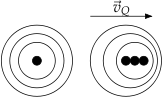
\includegraphics[width=3cm]{./bilder/doppler.png}\\
		Ruhende \& bewegte Punktquelle \\ \\ \\
		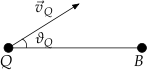
\includegraphics[width=3cm]{./bilder/doppler-bewegte-quelle.png}\\
		Bewegte Punktquelle \\ \\ \\
		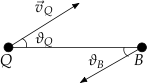
\includegraphics[width=3cm]{./bilder/doppler-beide-bewegt.png} \\
		Bewegter Beobachter \& bewegte Quelle \\
		\end{minipage}
	& \begin{minipage}[]{7cm}
      	\renewcommand{\arraystretch}{2}
      	\vspace{.2cm}
	  	\textbf{Bewegte Quelle, ruhender Beobachter} \\
	  	$f_B = \dfrac{1}{1 \mp  \dfrac{v_Q}{u}} f_Q$ \qquad \parbox{3cm}{- auf Hörer zu \\
	  				 + von Hörer weg}\\
	  	$f_B = \dfrac{1}{1 - \dfrac{v_Q}{u} \cos(\vartheta_Q)} f_Q$ \\
	  	\vspace{.5cm}\\
	  	\textbf{Ruhende Quelle, bewegter Beobachter} \\
	  	$f_B = \left(1 \pm \dfrac{v_B}{u}\right) f_Q$ \qquad + auf Quelle zu \\
	  	$f_B = \left(1 + \dfrac{v_B}{u} \cos(\vartheta_B)\right) f_Q$ \\
	  	\vspace{.5cm}\\
	  	\textbf{Allgemein} \\
	  	$f_B = \dfrac{u + v_B \cos(\vartheta_B)}{u - v_Q \cos(\vartheta_Q)} f_Q$ \\
	  	\vspace{.5cm}\\
	  	\textbf{Optischer (transversaler) Dop.-Effekt } \\
	  	$f_B = \dfrac{\sqrt{1 - \beta^2}}{1 - \beta \cos \vartheta_{rel}} f_Q \qquad \beta =
	  	\dfrac{v_{rel}}{c}$ \\ 
	  	$ \vec{v}_{rel} = \vec{v}_B - \vec{v}_Q \vspace{.5cm}\\
	  	\textbf{Schwebungsfrequenz}\\
	  	\Delta f = |f_{Empfangen} - f_{Gesendet}|$ \vspace{.2cm}
      	\renewcommand{\arraystretch}{1}
    	\end{minipage}
	& \parbox{6.5cm}{
		$f_B \;$ gehörte Frequenz \\
		$f_Q \;$ gesendete Frequenz \\
		$v_B \;$ Geschwindigkeit Beobachter \\
		$v_Q \;$ Geschwindigkeit Quelle\\
		$u \;$ Schallgeschwindigkeit\\
		$v_{rel} \;$ Relativgeschwindigkeit zw. Q und B\\
		$\vartheta_{rel} \;$ Winkel zwischen $\vec{v}_{rel}$ und $\overline{BQ}$
		} \\
\hline
\end{tabular}

\begin{minipage}{10cm}
	\subsection{Machscher Kegel \kuchling{344} \stoecker{278}}
	\begin{tabular}{ll}
	\parbox{5cm}{
		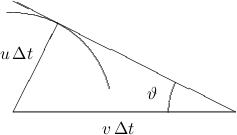
\includegraphics[width=4cm]{./bilder/machscher-kegel.png}}
		& 
		\parbox{5cm}{$\sin(\vartheta)=\dfrac{u}{v} = \dfrac{1}{M}$ \\ \\
		Machzahl: $M=\dfrac{v}{u}$}
	\end{tabular}
\end{minipage}
\begin{minipage}{8cm}
	\subsection{Lichtwellen}
		Lichtgeschwindigkeit: $ c = \dfrac{1}{\sqrt{\mu_0 \cdot \epsilon_0}} \qquad \qquad$ \\
		Intensität: $I = \dfrac{1}{2} \cdot \sqrt{\dfrac{\epsilon_0}{\mu_0}} \cdot {E_0}^2 \quad$ in $[W/m^2]$
\end{minipage}


\subsection{Optische Länge}
Durchqueren Wellen Medien, muss mit optischen Längen gerechnet werden.\qquad 
$s$ wird zu $n\,s$ \qquad $\lambda$ wird zu $\dfrac{\lambda}{n}$



\subsection{"Uberlagerung / Interferenz \kuchling{233, 235} \stoecker{272, 354}}
\setlength{\tabcolsep}{5pt}
\renewcommand{\arraystretch}{2}
\subsubsection{Interferenzbedingungen}
\begin{tabular}{p{11cm} p{7cm}}
\begin{minipage}[]{11cm}
	\begin{tabular}{|l|l|l|}
	\hline
	& \textbf{Phase} & \textbf{Weg} \\
	\hline
	Konstruktiv: 
		& $k_0(n\cdot \Delta x)=m \, 2\pi$
		& $n \, \Delta x = m \, \lambda$ \\
	Destruktiv: 
	 	& $k_0(n\cdot \Delta x)=(2m+1)\pi$
	 	& $n \, \Delta x = (2m+1) \frac{\lambda}{2}$ \\
	\hline
	\end{tabular}\\
	\end{minipage}
	& \parbox{8cm}{$k_0 = \dfrac{2\pi}{\lambda_0}$ = Wellenzahl im Vakuum\\
	$ \lambda_0$ = Wellenlänge im Vakuum\\
	n = Brechungsindex, Kuchling Tab 39, S.653\\
	$n\cdot \Delta x$ = optische Gangdifferenz}
\end{tabular}\\
\textbf{Phasensprung:}
		\parbox{16cm}{Ein Phasensprung um $\pi$ bzw. $\frac{\lambda}{2}$ findet bei
		\textbf{Reflektion} an einem härteren oder optisch dichterem Material
		(\textbf{höheres $n$}) statt.}
		
\subsection{Remission/Transmission}
\textbf{Remission} $R= \left(\dfrac{f-1}{f+2}\right)^2$ mit $ f = \dfrac{n_1}{n_2}$\hspace{2cm} \textbf{Transmission} $T = 1-R$  

\subsection{Schallmessung \kuchling{348} \stoecker{287}}
\setlength{\tabcolsep}{5pt}
\renewcommand{\arraystretch}{2.4}
\begin{tabular}{>{\bfseries}ll}
Welle: & $\xi=\xi_0\sin(\omega t-kx)$ \qquad $\xi_0$ Schallausschlag \qquad
$[\xi]$: m
\\
Schallschnelle: & $v=v_0\cos(\omega t-kx)\qquad\rightarrow\qquad v=\dot{\xi}=\omega\xi_0\cos(\omega t-kx)\rightarrow \dfrac{v_0}{\omega}=\xi_0$\\
Schall(wechsel)druck: & $\tilde p=\Delta p_0 \cos(\omega t-kx)$ \\
Druckamplitude: & $\Delta p_0=Z\cdot v_0$ \qquad Schallimpedanz $Z=\varrho
\cdot u$\\ 
Effektivwert: & $p_{\text{eff}} = \dfrac{\Delta p_0}{\sqrt{2}}$\\
Schallintensität: & $I=\dfrac{1}{2}\,\varrho\, v_0^{\,2}\,u =
\dfrac{1}{2}\varrho\,\omega^2\, \xi_0^{\,2}\,u =  \dfrac{\Delta
p_0^{\,2}}{2\cdot Z}$ \qquad $\xi_0$ Schallausschlag; $\varrho$ Dichte des Mediums\\  

Schallpegel [dB] : & $\boxed{L_I=10\cdot \log\left(\dfrac{I}{I_0}\right)}$\qquad
$I_0=10^{-12}$ W/m$^2$ \qquad $L_I=L_p$ f"ur Z=400kg/m$^2$s @ 20$^{\circ}$C\\
Schalldruckpegel: & $L_p=20\cdot\log\left(\dfrac{p_{\text{eff}}}{p_{\text{eff}_0}}\right)= 20\cdot\log\left(\dfrac{\Delta p_0}{\sqrt{2}\cdot p_{\text{eff}_0}}\right)$\qquad $p_{\text{eff}_0}=2\cdot 10^{-5}$ Pa\\
Schallschnellenpegel: & $L_v=20\cdot\log\left(\dfrac{v_{\text{eff}}}{v_{\text{eff}_0}}\right)$ \qquad $v_{\text{eff}_0}=5\cdot10^{-8}$m/s \\
Schallleistungspegel: & 
$L_P = 10\cdot\log\left(\dfrac{P}{P_0}\right)$ \qquad  $P_0=10^{-12}$W\\
Schallfluss: & $\vec q=\int\limits_{A}{\vec v\cdot dA}$\\
Wellengeschwindigkeit: & $u=\sqrt{\dfrac{1}{\varrho\,\kappa}}=\underbrace{\sqrt{\dfrac{\varkappa\,p}{\varrho}}=\sqrt{\dfrac{\varkappa\,R\,T}{M}}}_{\text{f"ur Gase}}$ \qquad (Schallgeschwindigkeit) $\kappa$: Kompressibilit"at \quad\\
& $\Rightarrow\dfrac{\Delta V}{V}=-\kappa\cdot\Delta p$ \qquad ($p\cdot V=\text{const}\,\,@\,\,T_{\text{const}}$ bzw. $p\cdot V^{\varkappa}=\text{const}$) \\
Lautstärke: & $S=2^{0.1\cdot(L_S-40)}$ \qquad $L_S=$ Lautst"arkepegel [phon] = $L_P$ @ 1kHz, H"orschwelle 4phon\\
Ebene Welle & (z.B. Parabolspiegel) $\rightarrow$ konstantes I, keine geom. D"ampfung nur Luftd"ampfung\\
& $\boxed{L_2=L_1-K\cdot(r_2-r_1)}$ f"ur $d<<r\quad\rightarrow\quad$ $I_2=\dfrac{P}{4\pi(r+d)^2}\approx\dfrac{P}{4\pi r^2}=I_1$\quad$I=$konstant\\
\parbox{3cm}{Kugelwellen\\
(Punktquellen)}: &  $I=\dfrac{P}{4\pi r^2}\quad\rightarrow\quad \sim\dfrac{1}{r^2}$ und $\dfrac{I_2}{I_1}=\dfrac{r_1^{\,2}}{r_2^{\,2}}$  \\
&$\boxed
{L_2=L_1-\underbrace{20\cdot\log\left(\dfrac{r_2}{r_1}\right)}_{\text{geom. D"ampfung}}-\underbrace{K\cdot(r_2-r_1)}_{\text{Luftd"ampfung}}}$\quad mit $K$: Schalldämpfung [dB/m]\\
\parbox{3cm}{Zylinderwellen\\
(Linienquellen)}: &$I=\dfrac{P}{l\,2\pi r}\quad\rightarrow\quad \sim\dfrac{1}{r} \quad \Rightarrow \boxed{L_2=L_1-10\cdot\log\left(\dfrac{r_2}{r_1}\right)-K\cdot(r_2-r_1)}$ \\
Schalld"ammung: & $\boxed{R=10\,\log\left(\dfrac{P_1}{P_2}\right)}$ \\
Phasensprung & um $\lambda/2$, $\pi$ bei Reflexion w"ahrend "Ubergang von gasf"ormig $\rightarrow$ fest  \\
Infra-/Ultraschall & Infraschall $<$ 16Hz...20kHz $<$ Ultraschall ...10GHz $<$ Hyperschall\\
\end{tabular}
\renewcommand{\arraystretch}{\arraystretchOriginal}

\subsection{Wellenoptik}

\subsubsection{Prinzip von Huygens \kuchling{229}}
Jeder Punkt einer Welle ist Zentrum einer neuen Kugelwelle  
(sogenannte Huygens‘sche Elementarwelle). 
Die Wellenfront zu einem späteren Zeitpunkt ist die Einhüllende dieser Huygens'schen Elementarwellen.\\

\begin{minipage}{9.5cm}
	\subsubsection{Beugung am Doppelspalt}
	\begin{minipage}{4.5cm}
	\textbf{Minimum n-ter Ordnung}\\
		$\sin(\varphi_n) \cdot s = (2n + 1)\cdot \frac{\lambda}{2} $\\
	\textbf{Maximum n-ter Ordnung}\\
			$\sin(\varphi_n) \cdot s = n \cdot \lambda $\\ 
			\\
		\begin{minipage}{4.5cm}
			$\lambda$ = Wellenlänge des Lichts\\
			$s$ = Spalt-Abstand\\
			$\varphi_n$ = Winkel n-ter Ordnung\\
			$n$ = 0,1,2,... = Ordnung
		\end{minipage}
	\end{minipage}
	\begin{minipage}{4cm}
		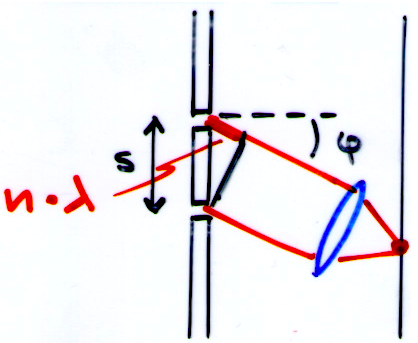
\includegraphics[width = 4cm]{./bilder/beugung-doppelspalt}
	\end{minipage}
\end{minipage}
\begin{minipage}{9cm}
	\subsubsection{Beugung am Einfachspalt}
	\begin{minipage}{4.5cm}
	\textbf{Minimum n-ter Ordnung}\\
		$\sin(\varphi_n) \cdot s = n \cdot \lambda $\\ 	
	\textbf{Maximum n-ter Ordnung}\\
		$\sin(\varphi_n) \cdot s = (2n + 1)\cdot \frac{\lambda}{2} $\\	
		\\
		\begin{minipage}{4.5cm}
			$\lambda$ = Wellenlänge des Lichts\\
			$s$ = Spalt-Abstand\\
			$\varphi_n$ = Winkel n-ter Ordnung\\
			$n$ = 0,1,2,... = Ordnung
		\end{minipage}
	\end{minipage}
	\begin{minipage}{4cm}
		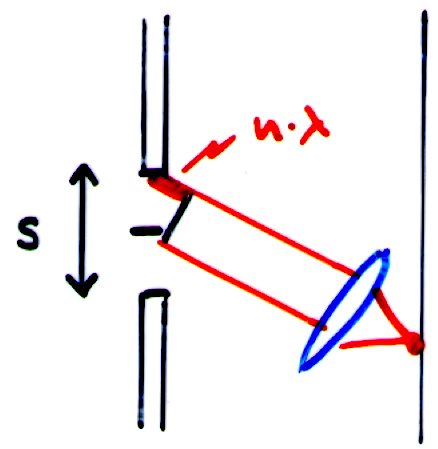
\includegraphics[width = 4cm]{./bilder/beugung-einfachspalt}
	\end{minipage}
\end{minipage}


\subsubsection{Beugung am Gitter}
\begin{minipage}{6cm}
	\textbf{Hauptmaximum n-ter Ordnung}\\
	$\boxed{\sin(\varphi_n) \cdot d = n \cdot \lambda}$\\
	\\
	\begin{minipage}{6cm}
		$\lambda$ = betrachtete Lichtwellenlänge\\
		$d$ = konstanter Spaltenabstand\\
		$\varphi_n$ = Maximumwinkel n-ter Ordnung \\
		$n$ = 0,1,2,... = Ordnung
	\end{minipage}
\end{minipage}
\begin{minipage}{5cm}
	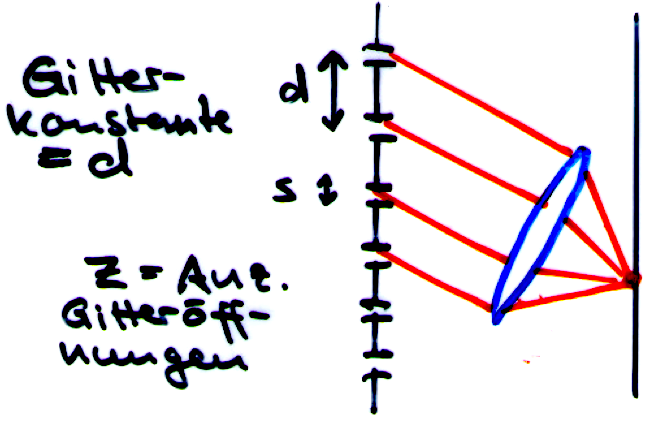
\includegraphics[width = 4cm]{./bilder/beugung-gitter}
\end{minipage}
\begin{minipage}{8cm}
	\textbf{Bedingungen für optimales optisches Gitter}
	\begin{enumerate}
		\item Möglichst kleine Gitterkonstante $\mathbf{d}$
		\item Möglichst grosse Gitter-Zahl $\mathbf{z}$
		\item Möglichst kleine Gitter-Breite $\mathbf{s}$
	\end{enumerate}
\end{minipage}\\
\\ \\
\begin{minipage}{18cm}
	\begin{tabular}{lllll}
	\parbox{4.5cm}{Intentitäts-Verteilung	\textbf{Gitter}}
		& $\approx$
		& \parbox{5.5cm}{Formfaktor\\
				{\small = Intensitätsverteilung \textbf{Einzelspalt}}}
		& $\times$
		& \parbox{6cm}{Interferenzfunktion\\
						{\small = Intensitätsverteilung \textbf{Doppelspalt}}}\\	
	\parbox{4.5cm}{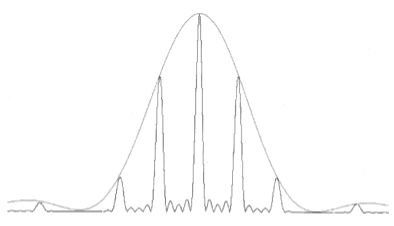
\includegraphics[width = 4.5cm]{./bilder/intensitaetsverteilung-gitter}}	
		& $\approx$
		& \parbox{4.5cm}{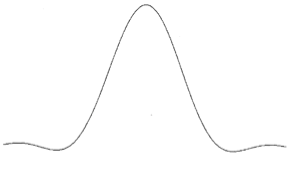
\includegraphics[width = 4.5cm]{./bilder/intensitaetsverteilung-einzelspalt}}
		& $\times$
		& \parbox{4.5cm}{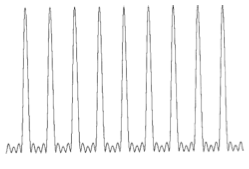
\includegraphics[width = 4.5cm]{./bilder/intensitaetsverteilung-doppelspalt}}
		\\			
	\end{tabular}
	Dabei entsteht immer z-2 Neben-Maxima.
\end{minipage}

\subsubsection{Babinet-Theorem}
Komplemetäre Strukturen (also Negativ und Positiv) liefern gleiche Beugungsbilder

\newpage

\input{idiotenseite/Idiotenseiteinclude}

\newpage

\section{Übungen}
\subsection{Wellenlänge}
Berechnen sie die Frequenz einer Radiowelle mit der Wellenlänge $\lambda$ von 5$00m$
\[
	f=\frac{c}{\lambda} = \frac{3\cdot 10^8m/s}{500 m} = 600kHz
\]

Ein Laser mit einer Frequenz von $4.5\cdot 10^{14} Hz$ und einer Leistung von $P=0.2mW$ sendet Photonen aus. Wieviele Photonen verlasen den Laser pro Sekunde.
\begin{itemize}
\itemsep0em
\item $h = $ Planksches Wirkungsquantum $=6.6\cdot 10^{-34}\frac{J}{Hz} = 6.6\cdot 10^{-34} Js$
\item $n = $ Anzahl Photonen
\end{itemize}
\begin{align*}
E= h\cdot f\\
E_{ges} &= n\cdot E\\
P&= \frac{E_{ges}}{t} = \frac{E\cdot n}{t}\\
n&=\frac{P\cdot t}{E\cdot n} = \frac{0.0002W\cdot 1s}{6.6\cdot 10^{-34}Js\cdot 4.5\cdot10^{14}Hz} \approx 6.7\cdot 10^{14}
\end{align*}

\subsection{Lichtbrechung}
Ein gelber Lichtstrahl mit einer Wellenlänge von $\lambda = 589 nm$ trifft unter einem Einfallswinkel $\alpha_1 = 25^\circ$ auf die Grenzfläche zwischen Wasser und Flintglas. Unter welchem Winkel wird
er von seiner ursprünglichen Richtung abgelenkt? Die Brechungsindizes bei $\lambda = 589 nm$ betragen:\\
\begin{tabular}{ll}
Wasser: &$n = 1.333$\\
Flintglas: &$n = 1.603$
\end{tabular}


\begin{minipage}{0.69\textwidth}
\begin{align*}
	\delta &= \varepsilon_1-\varepsilon_2\\
	n_1\cdot \sin(\varepsilon_1) &= n_2\cdot \sin(\varepsilon_2)\\
	\delta &= \varepsilon_1 - \arcsin\left(\frac{n_1}{n_2}\cdot \varepsilon_1\right)\\
	4.42^\circ&=-\arcsin\left(\frac{1.333}{1.603}\cdot \sin(25^\circ)\right)
\end{align*}
\end{minipage}
\begin{minipage}{0.3\textwidth}
	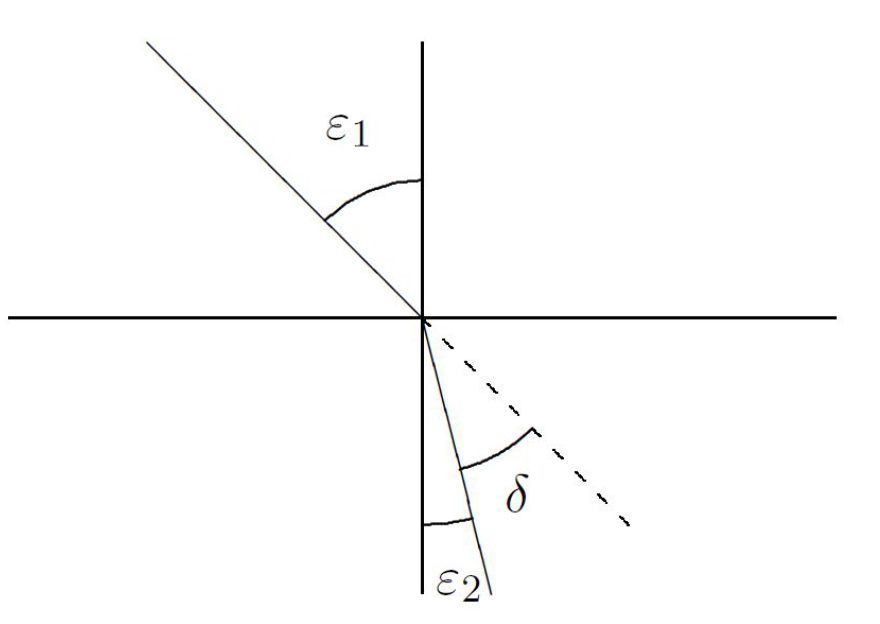
\includegraphics[width=0.9\textwidth]{bilder/lichtbrech.png}
\end{minipage}

\textbf{Spiegel}\\
Wie gross ist das Bild eines 4 cm grossen Gegenstands, der sich im Krümmungsmittelpunkt eines sphärischen Konkavspiegels mit einem Krümmungsradius von 50 cm befindet? Wie gross ist die Bilddistanz?
\[
	f=\frac{r}{2} = 0.25m\quad \frac{1}{f} = \frac{1}{b}+\frac{1}{g} \qquad b= \frac{1}{\frac{1}{f}-\frac{1}{g}} = \frac{1}{\frac{1}{0.25}- \frac{1}{0.5}} = 0.5m \qquad \frac{B}{G} = \frac{b}{g} \Rightarrow B= \frac{b\cdot G}{g} = \frac{0.5\cdot 0.04}{0.5} = 0.04m = 4cm
 \]
Wobei: \begin{itemize}
			\itemsep0em
			\item $f$ = Brennweite
			\item $g$ = Gegenstandsweite (Abstand vom Spiegel zum Gegenstand)
			\item $b$ = Bildweite (Abstand vom Spiegel zum Bild)
			\item $B$ = Bildgrösse
			\item $G$ = Gegenstandsgrösse
\end{itemize}

\textbf{Kamera und Spiegel}
Ein Fotoamateur fotografiert in einem Reisebus Personen der Reisegesellschaft über den Innenrückspiegel des Fahrers. Die Kamera ist $1m$ vom Rückspiegel entfernt. Um das Bild von Passagieren, die sich 1.5 m hinter der Kamera befinden, scharf zu erhalten, muss der
Amateur das Objektiv auf eine Distanz von 1.8 m einstellen. Wie gross ist die Brennweite des Rückspiegels?

\begin{minipage}{0.39\textwidth}
\[
	b = a-d =-0.8m\qquad g = a+c = 2.5m
\]
\[
	f=\frac{1}{\frac{1}{g}+\frac{1}{b}} = \frac{1}{\frac{1}{2.5m}+\frac{1}{(-0.8m)}} = -1.18m
\]
\end{minipage}
\begin{minipage}{0.59\textwidth}
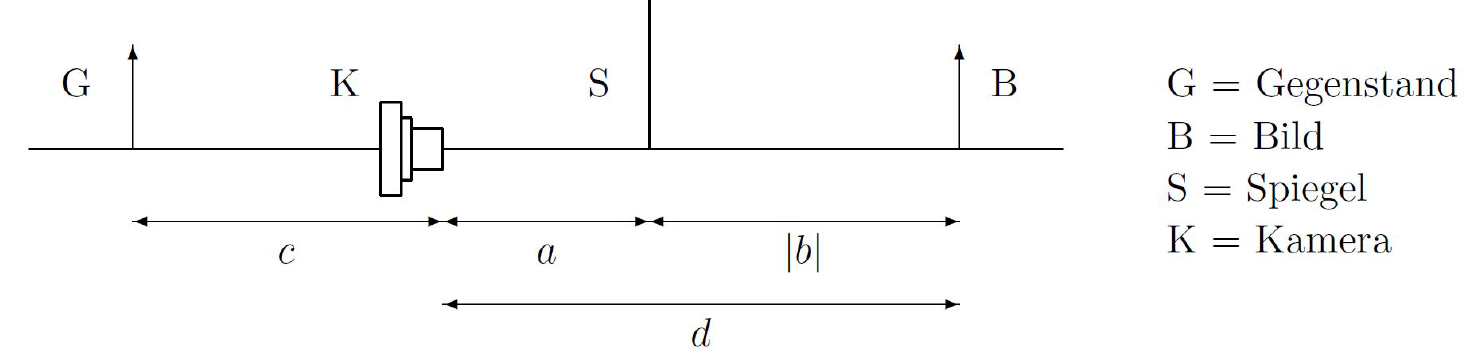
\includegraphics[width=0.99\textwidth]{bilder/a31.png}
\end{minipage}

\textbf{Kamera I}\\
Ein Fotoobjektiv mit einer Brennweite von 50 mm ist in einer Gewindefassung mit einer Ganghöhe von 4 mm in eine Kamera eingebaut. Wie gross ist der Drehwinkel zwischen
den Entfernungseinstellmarken für 3 m und 5 m?
\[
	\Delta b = b_1-b_2 = \left(\frac{1}{\frac{1}{f}-\frac{1}{g_1}}-  \frac{1}{\frac{1}{f}-\frac{1}{g_2}}\right) = \left(\frac{1}{\frac{1}{0.05}-\frac{1}{3}}-\frac{1}{\frac{1}{0.05}-\frac{1}{5}}\right) = 0.3424mm\qquad \alpha = \frac{\Delta b}{h} \cdot 360^\circ = \frac{0.3424mm}{4mm}\cdot 360^\circ = 30.81^\circ
\]

\textbf{Kamera mit Unschärfe}\\
Ein Fotoamateur will einen Motorradfahrer, der mit einer Geschwindigkeit von $v=72 km/h$ vorbeifährt, aus $g=10m$ Distanz von der Seite fotografieren. Sein Fotoapparat hat ein
Objektiv mit $f=50 mm$ Brennweite. Welche Belichtungszahl muss er einstellen, damit die
Bewegungsunschärfe auf dem Film höchstens 0.1 mm wird?\\
Die Bewegungsunschärfe kann als Bildgrösse $B$ interpretiert werden!
\begin{align*}
	b&= \frac{1}{\frac{1}{f}-\frac{1}{g}} \textrm{ da f }<< g \Rightarrow b\approx f\\
	G&= \frac{g\cdot B}{b} \quad \textrm{und} \quad G=v\cdot t \quad \Rightarrow v\cdot t = \frac{g\cdot B}{b}\\
	t&= \frac{g\cdot B}{f\cdot v} = \frac{10m \cdot 0.1mm}{0.05mm \cdot 20m/s}= \frac{1}{1000}s
\end{align*}

\textbf{Kamera mit Unschärfe II}\\
Das $f=35mm$ Objektiv eines Fotoapparates ist auf $g_0= \infty$ eingestellt. Wie nahe darf ein Gegenstand sein, damit bei einer Blendenöffnung von $q=1/16$ die Unschärfe des Bildes kleiner als $2\cdot 10^{-5}$m ist?
\begin{align*}
\frac{1}{g} &= \frac{1}{g_0} \pm \frac{u}{qf^2}  \\
g&=\frac{1}{\frac{1}{g_0} \pm \frac{u}{qf^2}} \quad \textrm{da }g_0= \infty \Rightarrow g= \frac{qf^2}{u} = \frac{1\cdot (0.035)^2}{16\cdot 2\cdot 10^{-5}} = 3.828m
\end{align*}

\textbf{Fernrohr}
Ein Turm von 40 m Höhe wird aus einer Entfernung von $g=12km$ durch ein astronomisches Fernrohr betrachtet, dessen Objektiv eine Brennweite $f_1=150cm$ und dessen Okular eine Brennweite $f_2=5 cm$ aufweist. Welche Distanz müssen die beiden Linsen voneinander
haben, wie gross ist die Vergrösserung, und unter welchem Sehwinkel erscheint der Turm im Fernrohr? Wie gross ist die Austrittspupille, und in welchem Abstand vom Okular befindet sie sich, wenn das Fernrohr eine Lichtstärke von $L=25$ aufweist? Wie gross ist der
Durchmesser des Objektivs?

\begin{align*}
l &= f_1+f_2 = 150cm+5cm = 155cm\\
V &= \frac{f_1}{f_2} =\frac{150}{5} = 30\\
\varepsilon&= \arctan\left(\frac{B}{f_2}\right) \quad B = \frac{b\cdot G}{g}\quad b= \frac{1}{\frac{1}{f_1}-\frac{1}{g}} \approx f_1\\ 
\varepsilon&= \arctan\left(\frac{f_1\cdot G}{g\cdot f_2}\right) = \arctan\left(\frac{1.5\cdot 40}{12'000\cdot 0.05}\right) = 5.71^\circ
\end{align*}




\newpage
\subsection{Ungedämpfte Schwingungen}
\textbf{Harmonische Schwingung 1}\\
Eine harmonische Schwingung ist durch folgende Anfangsbedingungen gegeben: Die Auslenkung $A=2cm$ zum Zeitpunkt $t = 0$s. Die Geschwindigkeit $u_0 = -2cm$ zum Zeitpunkt $t = 0$. Die Schwingung hat eine Periode $T=2s$. Durch diese Angaben ist der weitere Verlauf
der Schwingung eindeutig bestimmt. Berechnen Sie die harmonische Funktion, die diese Schwingung beschreibt.

\begin{align*}
y(0) &=s_0 =  2cm\quad \dot{y}(0) = u_0 = -2cm\\
y(t = 0) &= A \cdot \sin(\omega \cdot 0 + \varphi) = s_0\\
\dot{y}(t = 0) &= \omega \cdot  A \cdot \cos(\omega \cdot 0 + \varphi) = v_0\\
A\cdot \sin(\varphi) &= s_0\\
A\cdot \cos(\varphi) &=\frac{v_0}{\omega}\\
&\textrm{ 2 Gleichungen} \Rightarrow \textrm{ solve!}
\end{align*}

\textbf{Mathematisches Pendel}\\
Die an einem Baukran knapp über dem Boden hängende Last pendelt langsam hin und her. Eine Schwingung dauert 15.6 s. Wie hoch ist der Kran?
\[
	T= 2\pi\sqrt{\frac{l}{g}}\Rightarrow l=\frac{gT^2}{4\pi^2} = \frac{9.81\cdot (15.6s)^2}{4\pi^2} = 60.47m
\]

\subsection{Gedämpfte Schwingungen}
\textbf{1. Logarithmisches Dekrement}\\
Wie gross ist das logarithmische Dekrement der gedämpften harmonischen Schwingung eines Massenpunktes, wenn dieser in $10s$ $50\%$ seiner mechanischen Energie verliert und die Schwingungsdauer $0.2s$ beträgt?
\begin{align*}
	\frac{E_2}{E_1} &= \frac{(A_2)^2}{(A_1)^2} = 0.5\\
	A_1&=\sqrt{2}\cdot A_2\\
	\frac{A_1}{A_2} &= \sqrt{2}=e^{\delta t}\\
	\delta \cdot t&= \ln(\sqrt{2})\\
	\Lambda&=\delta T = \frac{\ln(\sqrt{2})\cdot T}{t}=\frac{\ln(2)\cdot 0.2s}{10s}=6.93\cdot 10^{-3}
\end{align*}

\textbf{2. Logarithmisches Dekrement}\\
Das logarithmische Dekrement einer gedämpften Schwingung beträgt $\Lambda = 1.1$. Um wieviel unterscheidet sich die Eigenfrequenz der gedämpften Schwingung von der ungedämpften Schwingung?
\begin{align*}
\delta &= \frac{\Lambda}{T}\\
\omega&=\sqrt{\omega_0^2-\delta^2}=\sqrt{\left(\frac{2\pi}{T}\right)^2-\left( \frac{\Lambda}{T}\right)^2}\\
\frac{\omega}{\omega_0}&= \frac{\frac{2\pi}{T}}{\sqrt{\left(\frac{2\pi}{T}\right)^2-\left(\frac{1.1}{T} \right)^2}} = 1.01568\\
\%&= ans\cdot 100\%-100\% = 1.568\%
\end{align*}






\subsection{Motor mit Unwucht}
\begin{minipage}{0.49\textwidth}
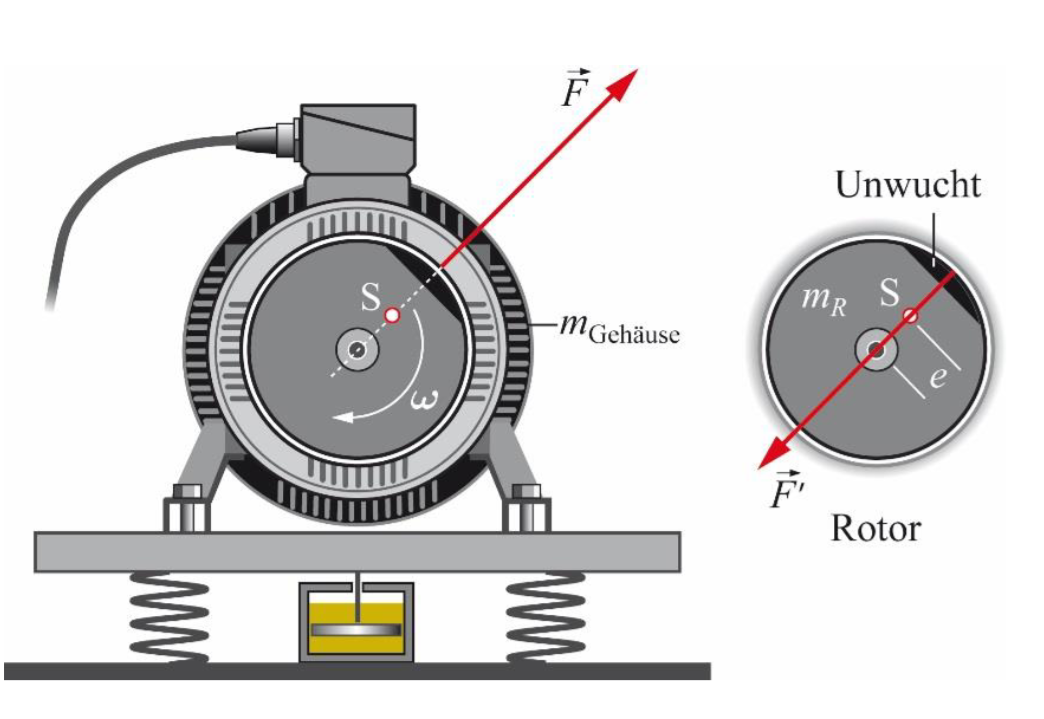
\includegraphics[width=0.8\textwidth]{bilder/motor_unwucht.png}
\end{minipage}
\begin{minipage}{0.49\textwidth}
\begin{align*}
D&=0.1\\
M_{tot} &= 300kg\\
m&= 30kg\\
M&= 270kg\\
f_e&= \textrm{ Kraft zwischen Rotor und Stator}\\
e&= 5mm = \textrm{Exzentrizität}\\
\omega  &= 2\pi f = \frac{2\pi\cdot 1500}{60\frac{s}{min}} = 50\frac{\pi}{s} = 157.08\\
k&= 500\frac{N}{cm} = 50'000\frac{N}{m}
\end{align*}
\end{minipage}

\[
	\begin{array}{rll}
		I&M\ddot{y} &= -k y -b\dot{y} +f_e\\
		II&m(\ddot{y}-\omega^2 e\cdot\sin(\omega t))&=-f_e\\
		I+II&(M+m)\ddot{y} - me\omega^2 \cdot \sin(\omega t) &=-ky-b\dot{y}\\
		& M_{tot} \ddot{y} +b\dot{y} + ky &= m e\omega^2 \cdot \sin(\omega t)\qquad \qquad \textrm{Standartlösung}\\
		&\omega_0 &=\sqrt{\frac{k}{M_{tot}}} = \sqrt{\frac{50'000}{300}} = 12.9\frac{rad}{s}\\
		&f_0 = \frac{\omega_0}{2\pi} = 2.05\frac{1}{s}&f_m = \frac{1500}{60} = 25\frac{rad}{s}	\\
		&\eta = \frac{\omega}{\omega_0} = \frac{157.08}{2.05} = 12.17\\
		&F_0=\underset{\textrm{Kraft Boden ohne Federn}}{m\cdot e\cdot \omega^2}  &= 30kg\cdot 0.005m\cdot (157.08)^2 = 3701N\\[1em]
		\textrm{Oder gemäss \ref{Unwucht} S. \pageref{Unwucht}}& F_{B0}=\dfrac{m_R\,e\,\omega^2\,\sqrt{1+4D^2\eta^2}}{\sqrt{(1-\eta^2)^2+4D^2\eta^2}}\\
		&=\frac{30kg\cdot 0.005\cdot (157.08)^2\cdot \sqrt{1+4\cdot 0.1^2\cdot 12.17^2}}{\sqrt{(1-12.17^2)^2+4\cdot 0.1^2\cdot 12.17^2}} &= 65.76N
	\end{array}
\]


\subsection{Gleichmässig beschleunigte Masse an Feder}
Eine Masse mit der Masse $m=0.1kg$ hängt an einer ungespannten Feder der Länge $l=0.5m$ mit der Federkonstante $k=10N/m$. Zum Zeitpunkt $t=0$ beschleunigt der Aufhängepunkt der Feder mit einer Konstanten Beschleunigung $a=2m/s$ nach oben.
\begin{align*}
	y(0) &=\frac{-mg}{k} = \frac{-0.1\cdot 9.81}{k} = -0.0981m\\
	\dot{y}(0) &= 0\\
	m\cdot \ddot{y}+k\cdot y &= 0 \Rightarrow y_H = A\cdot \sin(\omega t +\varphi)\\
	m\cdot \ddot{y}+k\cdot y &=\frac{1}{2} a t^2-mg\qquad \textrm{ Ansatz:}\quad yp=c_0+c_1\cdot t +c_2\cdot t^2\\
	\textrm{eingesetzt }\quad &2\cdot m\cdot c_2+k(c_0+c_1\cdot t +c_2\cdot t^2)=k\cdot \frac{1}{2}\cdot a\cdot t^2 -m\cdot g\\
	\textrm{Koeffizientenvergleich}\quad &k\cdot c_2 = \frac{1}{2} \cdot k\cdot a\\
	&c_2 = \frac{a}{2}\\
	&c_1=0\\
	&2m\cdot c_2+k\cdot c_0 = -m\cdot g\\
	&c_2 =\frac{-m\cdot g}{k}-\frac{m\cdot a}{k}\\
	\textrm{eingesetzt}\quad &y(t) = A\cdot \sin(\omega t +\varphi) -\frac{mg}{k}-\frac{ma}{k}+\frac{a}{2} t^2\\
	\textrm{Anfangswerte:}\quad t=0\quad &A\sin(\varphi) -\frac{mg}{k}-\frac{ma}{k} = \frac{-mg}{k}\\
	&A\sin(\varphi) = \frac{ma}{k}\Rightarrow A=\frac{ma}{k}\\
	&A\omega \cos (\omega t+\varphi) = 0 \Rightarrow \varphi = \frac{\pi}{2}\\
	y(t) &=0.02\sin\left(\frac{1}{10}t+\frac{\pi}{2}\right)-1.181+t^2
\end{align*}
\newpage
\subsection{Wellen}
\textbf{Doppelpendel}\\
\begin{minipage}{0.69\textwidth}
Betrachte zwei Kugeln, welche mit Federn verbunden sind (vgl. Abbildung). Die Kugeln
haben beide die Masse m, die Federn haben alle die Federkonstante k, und die ungespannten Längen sind $l = L /3$.
\[
	\begin{array}{l}
		m \ddot{y}_1 = -k(y_1-l) +mg + k(y_2-l-y_1)\\
		m \ddot{y}_2 = -k(y_2-l) +mg + k(y_2-l-y_1)\\
		\textrm{ Durch Addition ergibt sich}\\
		m(\ddot{y}_1 + \ddot{y}_2) = -k (y_1+y_2) +2mg +3kl\\
		\textrm{Definition der Schwerpunktskoordinaten } \;y_s = \frac{y_1 + y_2}{2}\\
		m(\ddot{y}_1 + \ddot{y}_2) = -k y_s +mg +\frac{3}{2} kl \Rightarrow \ddot{y}_s + \frac{k}{s} y_s = g +\frac{3}{2} \frac{kl}{m} \\
		y(s) = A_s\cdot \sin (\omega_s t+\varphi_s) +\frac{mg}{k} + \frac{3}{2} l  \qquad \omega_s = \sqrt{\frac{k}{m}}
		\textrm{ Durch Subtraktion ergibt sich:}\\
		m(\ddot{y}_1 -\ddot{y}_2 +3k(y_1 -y_2) = -3kl\\
		\textrm{Definition der Relativbewegung }\; y_d = y_1-y_2\\
		\ddot{y}_d +\frac{3k}{m}y_d =\frac{-3kl}{m}\\
		y_d =  A_D\cdot \sin(\omega_d t+\varphi_d) -l \quad \omega_d = \sqrt{\frac{3k}{m}}\\
		y_1(t) = y_s+\frac{y_d}{2} \qquad y_2 = y_s - \frac{y_d}{2}
	\end{array}
\]
\end{minipage}
\hfill
\begin{minipage}{0.29\textwidth}
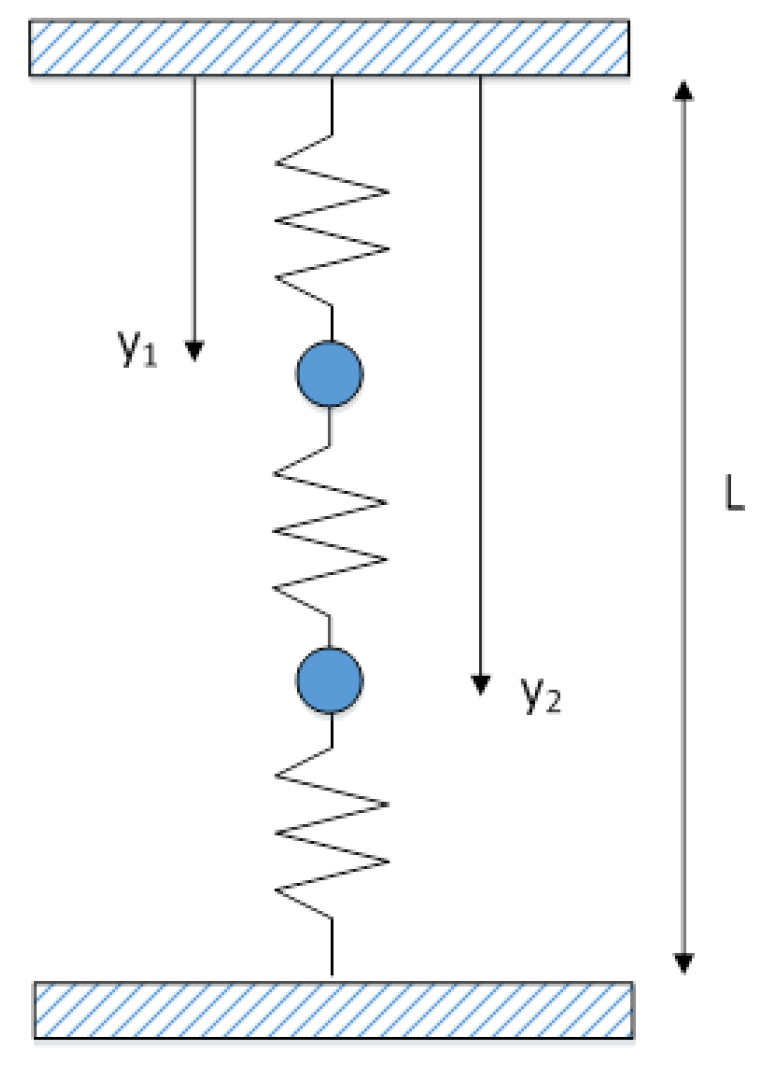
\includegraphics[width = 0.8\textwidth]{bilder/a91.png}
\end{minipage}





\textbf{Longitudinale Welle in Metallstab}\\
Ausbreitung der Geschwindigkeit einer Welle in einem Metallstab. (Der Stab wird auf die Kopfseite geschlagen, Longitudinale Welle).
\begin{align*}
E_{Stahl} &= 210GPa = \textrm{Elastitzizätsmodul}\\
\varrho_{Stahl} &= 7850 \frac{kg}{m^3}
m = \varrho A h \\
c &= E \frac{A}{h}\\
u^2 &= \frac{ch^2}{m} = \frac{(\frac{EA}{h})h^2}{\varrho A h} = \frac{E}{\varrho}  \Rightarrow u = \sqrt{\frac{E}{\varrho}} =\frac{2.1\cdot 10^11 Pa}{7850 \frac{kg}{m^3}} = 5172\frac{m}{s}
\end{align*}
\textbf{Schwingung einer Saite} (stehende Welle)\\
Eine Stahlseite der Länge $l=0.5m$. Die Saite ist fest eingespannt mit einer Zugkraft $F= 100N$ und einem Durchmesser $d=1mm$. Die Dichte der Stahlsaite ist $\varrho = 7850\frac{kg}{m^3}$
\begin{align*}
u&=2\cdot f \Rightarrow f = \frac{u}{2}\\
u&= \sqrt{\frac{F}{\varrho\cdot A}}\\
\lambda_1&= 2\cdot l = 2m\\
\lambda_n &= \frac{2\cdot L}{n}\\
A &= \pi\frac{D^2}{4} = \pi \frac{(10^{-3})^2}{4} = 7.85\cdot 10^{-7}m^2\\
u&= \sqrt{\frac{100N}{7850\cdot 7.85\cdot 10^{-7}}}=127.12 Hz
\end{align*}

\textbf{Stehende Welle in einem Rohr} (Bierflaschengrundton)

Ein Rohr mit einem offenen Ende (Bsp. Bierflasche) hat den Grundton $A = 440Hz$ Wie lang ist das Rohr bei $T = 293K$? Wie müsste man die Temperatur im Rohr ändern um eine Frequenz von $415.3Hz$ zu erzeugen.\\
\begin{align*}
L&=\frac{\lambda}{4} + n\frac{\lambda}{2}\quad \kappa= 1.4  \quad M=28.8\cdot 10^{-3}\frac{kg}{mol} \quad R=8.314\frac{J}{mol\cdot K}\\
u&=\sqrt{\frac{\kappa\cdot R\cdot T}{M}}=\sqrt{\frac{1.4\cdot 8.314\cdot 293}{29}}
\end{align*}

\textbf{Schwebung mit Klaviersaite}\\
$f_1 = 600Hz$, $f_2 = 606Hz$, $\Delta f = 6Hz$
\begin{align*}
u&=\sqrt{\frac{F}{\varrho\cdot A}}\\
f&=\frac{u}{2}\\
\lambda &= 2\cdot L\\
f_1&=\frac{1}{\lambda}\sqrt{\frac{F_1}{\varrho\cdot A}}\\
\frac{f_1}{f_2} &= \sqrt{\frac{F_1}{F_2}}\Rightarrow \frac{F_2}{F_1} = \left(\frac{f_2}{f_1}\right)^2 = \left(\frac{606Hz}{600Hz}\right)^2 = \frac{1.0201}{1}
\end{align*}



\textbf{Dopplereffekt}
\textbf{Frequenzvergleich}\\
Ein Auto fährt hupend mit einer Geschwindigkeit von 111 km/h dicht an einem ruhenden Beobachter vorbei. Um wieviel ändert sich die Tonhöhe? Die Lufttemperatur beträgt $\vartheta = 14.3^\circ C$, die mittlere Molmasse der Luft: $M=0.02883 g/mol$, der Adiabatenexponent der Luft: $\kappa = 1.4$\\
\begin{align*}
u&= \sqrt{\frac{\kappa R T}{M}} = \sqrt{\frac{1.4\cdot 8.3145\cdot (273.15+14.3)K}{0.02883}} = 340.676m/s\\
f_1 &= \frac{1}{1-\frac{v}{u}}\cdot f\\
f_2 &= \frac{1}{1+\frac{v}{u}}\cdot f\\
\frac{f_1}{f_2} &= \frac{\frac{1}{1-\frac{v}{u}}}{\frac{1}{1+\frac{v}{u}}} = \frac{\frac{1}{1-\frac{111/3.6}{340.676}}}{\frac{1}{1+\frac{111/3.6}{340.676}}} = 1.199
\end{align*}
\textbf{Bewegte Quelle und bewegter Beobachter}\\
Auf einer Strasse, die dicht an einer Bahnlinie entlang führt, fährt ein Motorradfahrer mit einer Geschwindigkeit $v_B =  90 km/h$. Ein Zug kommt ihm mit $v_Q =  120 km/h$ entgegen. Die Lokomotive pfeift mit einer Frequenz $f_q$ von 1000 Hz. Welche Frequenz hat der Ton, den
der Motorradfahrer hört? Die Schallgeschwindigkeit beträgt 343 m/s.
\[
f_B = \frac{u+v_B \cos(\vartheta_B)}{u-v_Q \cdot \cos(\vartheta_Q)}\cdot f_q = \frac{343+(90/3.6)m/s}{343-(120/3.6)m/s} \cdot 1kHz = 1188.4Hz
\]


\begin{minipage}{0.59\textwidth}
\textbf{Machscher Kegel}\\
Ein Geschoss fliegt mit der Geschwindigkeit $v = 660 m/s$ in einem Abstand $a=5m$ an einem Mann vorbei. Wie weit ist das Geschoss vom Mann entfernt, wenn er es hört? Schallgeschwindigkeit $u = 329.6m/s$
\begin{align*}
\sin(\vartheta) &= \frac{u}{v} = \frac{a}{d}\\
d&=\frac{v\cdot a}{u} = \frac{660\cdot 5}{329.6} = 10.01\frac{m}{s}
\end{align*}
\end{minipage}
\begin{minipage}{0.4\textwidth}
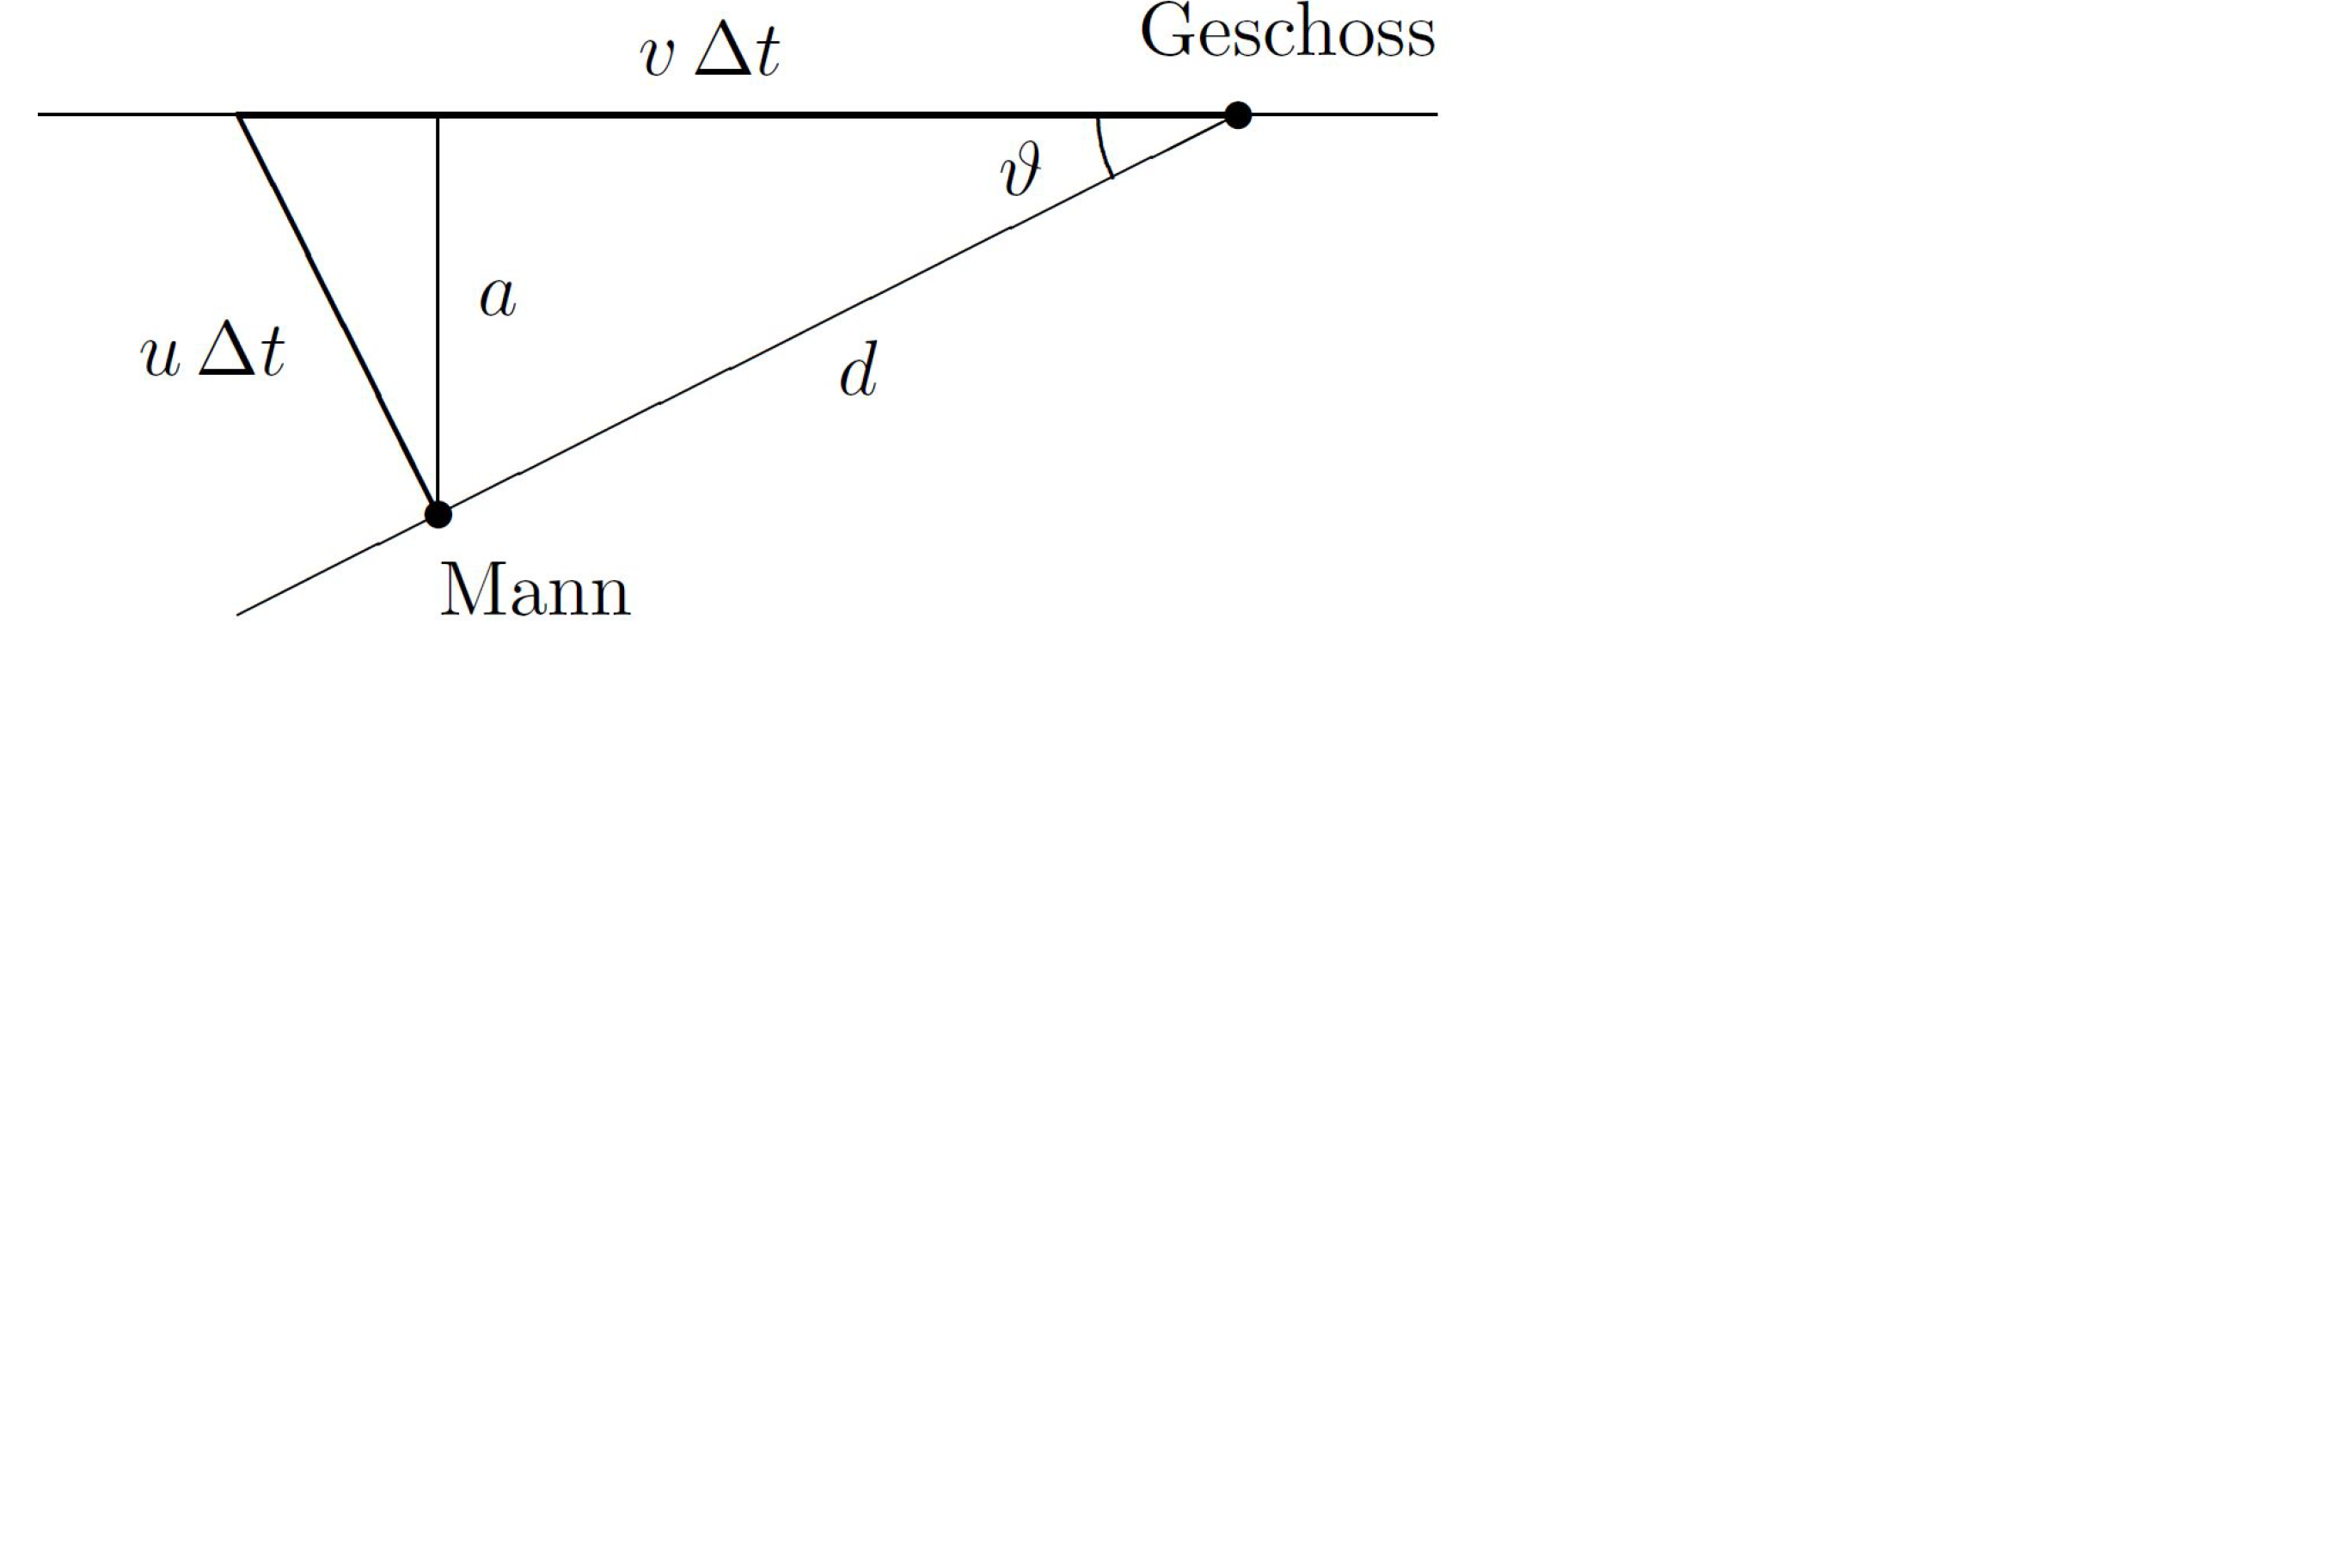
\includegraphics[width = 0.99\textwidth]{bilder/a113.png}
\end{minipage}

\textbf{Radarfalle}
Einem Auto wird von hinten unter einem Winkel $\vartheta = 160^\circ$ zur Fahrtrichtung ein Radarsignal mit der Frequenz $f_s = 1.8 GHz$ nachgesandt. Das reflektierte Signal wird mit der Senderfrequenz
 überlagert und erzeugt eine Schwebungsfrequenz $f_{\textrm{schweb}}  = 240 Hz$. Wie schnell fährt das Auto?\\

Aus der Formel $f' = \frac{\sqrt{1-\beta^2}}{1-\beta \cos(\vartheta)}\cdot f_s$ mit $\beta = \frac{v}{c}$ und mit $c= $ Lichtgeschwindigkeit $= 299'792'458 m/s$ lässt sich für Verhältnismässig kleine $v$ folgende Gleichung herleiten
\[
	\beta =\frac{v}{c} = \frac{-v_{\textrm{schweb}}}{2\cos(\beta)\cdot f_s} \Rightarrow v= \frac{-v_{\textrm{schweb}}\cdot c}{2\cos(\beta)} = \frac{-240\cdot 299'762'458}{2\cos(160)} = 21.267m/s = 76.56km/h
\]

\newpage

\textbf{Beispiel Interferenz mit Schallwellen}\\
Zwei Schallquellen schwingen in Phase mit der Amplitude $p_0$. An einem Punkt der sich $s_1 = 5m$ von der ersten Quelle und $s_2 = 5.17m$ von der zweiten Quelle entfernt befindet ist die Amplitude der Welle zu bestimmen die Frequenz $f = 500 Hz$ die Schallgeschwindigkeit $u= 340m/s$

\begin{minipage}{0.6\textwidth}
\begin{align*}
	\Delta x &= s_1-s_2 = 0.17m\\
	\lambda&= \frac{u}{f} = \frac{340m/s}{500} = 0.68m = 4\cdot \Delta x\\
	\delta &= \frac{2\pi\cdot \Delta x}{\lambda} = \frac{\pi}{2}\\
	p&= 2\cdot p_0 \cdot \cos\left(\frac{\delta}{2}\right)\\
	&= 2\cdot p_0\cdot \cos \left(\frac{\pi}{4}\right) = \sqrt{2} \cdot p_o	
\end{align*}
\end{minipage}
\begin{minipage}{0.39\textwidth}
Wobei:\\
$p_0 = $ Amplitude der Schallquelle\\
$p = $ Amplitude am Messpunkt\\
$\delta = $ Phasendifferenz am Messpunkt\\

\end{minipage}



\subsection{Lichtbeugung}
Es wird Licht mit einer Wellenlänge $\lambda = 633nm$ auf eine CD gestrahlt. Der Abstand zwischen den Maxima $x=1.25m$ auf einer Wand im Abstand $l=2.9m$. Wie gross ist der Abstand der Spuren auf der CD
\begin{align*}
\varphi &=\arctan\left(\frac{x}{l}\right) = \arctan\left(\frac{1.25m}{2.9m}\right) = 23.317^\circ\\
d&=\frac{\lambda}{\sin(\varphi} = \frac{633nm}{\sin(23.317^\circ)} = 1.599\mu m
\end{align*} 


\subsection{Reflexion}
Eine Schallwelle bewegt sich in einer Luftschicht mit $T_1=300K$ und trifft auf eine Luftschicht mit $t_2 = 280K$. Wieviel von Ihrer Intensität wird reflektiert, wieviel absorbiert.

\[
	R = \left(\frac{Z_1-Z_2}{Z_1+Z_2}\right)^2 \quad Z=\varrho	\cdot u \quad \varrho = \frac{p\cdot M}{R\cdot T} = \frac{p}{R_s\cdot T} \quad u=\sqrt{\frac{\kappa \cdot R\cdot T}{M}}
\]
Wobei:\\
\begin{itemize}
\itemsep0em
\item $R_S =$ Spezifische Gaskonstante von Luft $ = 287.058\frac{J}{kg\cdot K}$\\
\item $p = $ Luftdruck
\item $T = $ Absolute Temperatur
\item $\kappa = 1.4$ Adiabatenexponent
\item $\varrho = $ Luftdichte
\item $ u = $ Wellengeschwindigkeit
\end{itemize}
\newpage

\section{Schall}
\textbf{Sirene}
Eine Sirene emittiert eine Schallleistung von 100W gleichmässig in alle Richtungen. In welchem Abstand beträgt der Schallintensitätspegel 50dB. (Ohne Dämpfung)
\begin{align*}
I&=\frac{P}{4\pi r^2} \Rightarrow r = \sqrt{\frac{P}{4\pi I}}\\
L_I &= 10\log  \frac{I}{I_0} \Rightarrow I = I_0^{L_I/10}\\
r &= \sqrt{\frac{P}{4\pi I_0 \cdot 10^{L_I/10}}} = \sqrt{\frac{100}4\pi 10^{-12} \cdot 10^{50/10}}
\end{align*}

\textbf{Elektrischer Funke}\\
Ein elektrischer Funke überspringt eine gerade Linie von $L=10m$ und erzeugt einen Schallimpuls der Radial nach aussen abstrahlt. Die Leistung $P$ der Schallemission beträgt  $16kW$. Welche Intensität hat der Schall in einem Abstand von 12m?\\
Welche Leistung nimmt ein akustischer Detektor mit einer aktiven Fläche $A=2cm^2$ in einem Abstand $r_9=9m$ auf.

\begin{align*}
I&=\frac{P}{A} = \frac{P}{2\pi r L} = \frac{16kW}{2\pi 12m 10m} = 21.22\frac{W}{m}\\
P&=I\cdot A\\
I_9&=\frac{P}{A} = \frac{P}{2\pi r_9 L} = \frac{16kW}{2\pi 9m 10m} = 28.29\frac{W}{m^2}\\
P&= I_9\cdot A = 28.29\frac{w}{m^2} \cdot 2cm^2 \cdot \frac{m^2}{10'000 cm^2} = 5.66mW
\end{align*}

\textbf{Konzert vs Pressluft}\\
Ein Rockkonzert hat 46m vor der Bühne einen Schallpegel von $L_B = 120dB$ Ein Presslufthammer hat einen Schallpegel von $L_H = 92dB$. Welches Verhältnis haben die Schallintensitäten zueinander.
\begin{align*}
L&= (10db) \log\left(\frac{I}{I_0}\right)\\
\Delta L &=(10dB)\left(\log\frac{I_B}{I_H}\right) = (10dB) \log \frac{I_B}{I_H}\\
\Rightarrow 28dB &= (10dB) \cdot  \log\frac{I_B}{I_H}\\
\frac{I_B}{I_H} &= 10^{2.8} = 631
\end{align*}
\section{Prüfung HS15}
\subsection{Optik}

Man hat einen Konkavspiegel und einen Planspiegel.\\
Um die Brennweite des Konkavspiegels zu bestimmen wird eine Kerze zwischen Spiegel und Wand positioniert. Abstand Spiegel zur Wand $s_1 = b = 1.8m$, Abstand Kerze zur Wand $s_2 = 1.2m$. Es erscheint ein scharfes Bild der Kerze an der Wand. Wie gross ist die Brennweite?

\begin{align*}
g&= s_1-s_2 = 1.8m-1.2m = 0.6m\\
f&=\frac{g\cdot b}{g+b} = \frac{1.6\cdot 0.6m}{1.8m+1.6m}=0.45m
\end{align*}

Wo erscheint das Bild der Nase wenn wir den Planspiegel 15cm vor die Nase halten? Um was für ein Bild handelt es sich? Können wir das Bild deutlich sehen?

\begin{itemize}
	\itemsep0em
	\item Es gilt die Gleichung: $g=-b$ Daraus folgt das sich das Bild im Abstand $2g = 0.3m$ befindet.
	\item Planspiegel erzeugen bei einer einfachen Reflexion ein virtuelles und ein einseitig umgekehrtes (seitenverkehrtes) Spiegelbild
	\item Ja können wir, da sich das Bild mehr als 25cm vom Auge entfernt befindet.
\end{itemize}

Wo erscheint das Bild wenn man den Planspiegel durch einen Konkavspiegel ersetzt?
\begin{align*}
	b &= \frac{g\cdot f}{g-f} = -0.225m\\
	\frac{B}{G} = \frac{b}{g} &\Rightarrow B = G\cdot \frac{b}{g} = G\cdot \frac{-0.225m}{0.15m} = -G\cdot 1.5
\end{align*}
Daraus folgt, dass das Bild virtuell, um Faktor 1.5 vergrössert und aufrecht ist.

\subsection{Schwingung}
Ein gefederter Sitz $m=12.5kg$ schwingt unbelastet mit einer Periode $T_1 = 0.35s$ an einer Feder hin und her. Sitzt eine Person im Sitz ist die neue Periodendauer $T_2 = 0.9s$\\
Berechnen sie die Masse $m_a$ der Person. (Ungedämpft)
\begin{align*}
	m\ddot{x} &= -c\cdot x\\
	\omega_1&= \sqrt{\frac{c}{m}}\\
	\omega_1&= \frac{2\pi}{T_1} = \frac{2\pi}{0.35s} = 17.952 s^{-1}\\
	c&= m\cdot \omega_1^2 = 12.5kg\cdot 4028.41\frac{N}{m}\\
	\omega_2 &= \frac{2\pi}{T_2} = 6.981s^{-1}\\
	m_{tot} &=\frac{c}{\omega_2^2} = \frac{4028.41 \frac{N}{m}}{(6.981)^2} = 82.651kg\\
	m_2 &= m_{tot} - m_1 = 82.651kg-12.5kg = 70.153kg
\end{align*}

Mit welcher Arbeit $W$ muss der Sitz angeregt werden um eine Amplitude von 10cm zu erreichen?
\begin{align*}
	W&=\frac{1}{2} c\cdot x^2 = \frac{1}{2} 4028.41\frac{N}{m} \cdot (0.1m)^2 = 20.142J
\end{align*}

Welche maximale Geschwindigkeit erreicht der beladene Sitz
\begin{align*}
	x(t) &= A\sin(\omega t)\\
	\dot{x}(t) &= A\cdot \omega	\cdot \underbrace{\cos(\omega\cdot t)}_{\textrm{ maximal} =1}\\
	\dot{x}_{max} &= A\cdot \omega = 0.1m \cdot 6.981s^{-1} = 0.6981\frac{m}{s}
\end{align*}

Durch die Dämpfung gehen die Auslenkungen in $N=10$ Schwingungen auf $\frac{2}{3}$ des Anfangswertes zurück. Berechnen sie den Dämpfungsgrad
\begin{align*}
	x(t) &= A\cdot e^{-\delta t} \sin(\omega \cdot t)\\
	\omega &= \sqrt{\omega_0^2 -\delta^2}\\
	e^{-\delta \cdot 10T} &= \frac{2}{3}\\
	\delta &= \frac{1}{10\cdot T} \cdot \ln(\frac{3}{2} = 0.045\frac{1}{s}
\end{align*}

\subsection{Interferenz}
Eine Seifenblase erscheint mehrfarbig obwohl die Seife farblos ist. Die Brechzahl des Seifenfilms ist $n=1.42$\\
Wie erklärt sich die Farbe Magenta\\
Durch destruktive Interferenz werden die grünen Farbanteile eliminiert. Übrig bleiben die roten und blauen Anteile welche Magenta ergeben.\\
Welche Dicke $d$ muss der Seifenfilm mindestens haben, dass für eine Wellenlänge $\lambda = 530nm$ destruktive Interferenz auftritt. Dies unter senkrechtem Lichteinfall.
\begin{align*}
k\cdot 2d -\pi &= (2m+1)\pi \quad  \textrm{ oder } n \, \Delta x = (2m+1) \frac{\lambda}{2}\\
\Rightarrow \frac{2\pi}{\lambda} \cdot 2d&=  2\pi \cdot m\\
\lambda_n &= \frac{\lambda_0}{n} = \frac{530nm}{1.42} = 373.239nm\\
d&= \frac{\lambda_n}{2}  = \frac{373.239nm}{2} = 186.62nm
\end{align*}	  	

\subsection{Dopplerradar}
Um die Geschwindigkeit eines Autos zu messen wird ein Dopplerradar verwendet. Dazu werden Wellen mit einer Frequenz $f=24 GHz$ ausgesendet. Wie schnell ist das Auto bei einer Frequenzdifferenz $\Delta f = 5kHz$
\begin{align*}
	f_e &= \sqrt{\frac{1+\left(\frac{u}{c}\right)^2}{\left(1-\frac{u}{c}\right)^2}}\cdot f_s\\	
	\Delta f &= f_e-f_s = \sqrt{\frac{1+\left(\frac{u}{c}\right)^2}{\left(1-\frac{u}{c}\right)^2}}\cdot f_s -f_s
\end{align*}
	Womit nach der Geschwindigkeit gesolvet werden kann.
	
Es gibt noch die Buebetrickliformle (linearisiert) die in diesem Fall auch zum richtigen Resultat führt.
\[
	v = \frac{|f_e - f_s|}{2\cdot f_s}\cdot c = \frac{5kHz}{24GHz}\cdot 300'000'000 m/s = 31.25m/s
\]

Wäre das Auto auch für eine Sendefrequenz $f_s = 1MHz$ messbar?\\
Da $\lambda = \frac{c}{f} = 300m$ wäre das Auto unsichtbar für die Welle.

\subsection{Koppelschwingung}
Zwei parallele Pendel sind über eine Feder aneinander gekoppelt. Die Massen der Pendel seien gleich. Die Federkonstante gegeben. Der Winkel $\alpha$ definiert die Ruhestellung.

\begin{minipage}{0.69\textwidth}
\begin{align*}
J_a\cdot \ddot{\varphi}_1 &= -m_1 g a_1(\varphi_1 +\alpha_1 + c \cdot h(l_0+(H(\varphi_2-\varphi_1)))\\
J_a\cdot \ddot{\varphi}_2 &= -m_2 g a_2(\varphi_2 +\alpha_2 - c \cdot h(l_0+(H(\varphi_2-\varphi_1)))\\[1em]
&\textrm{ In der Ruhelage gilt:}\\
-&m_1g \alpha_1 a_1+c h l_0 =0\\
&m_2g \alpha_2 a_2-c h l_0 =0\\[1em]
&\textrm{Damit vereinfachen sich die Bewegungsgleichungen zu:}\\
\ddot{\varphi}_1 &= -\frac{m_1 g a_1}{J_1} \varphi_1 + \frac{ch^2}{J_1} (\varphi_2 - \varphi_1)\\
\ddot{\varphi}_2 &= -\frac{m_2 g a_2}{J_2} \varphi_2 + \frac{ch^2}{J_2} (\varphi_2 - \varphi_1)\\[1em]
&\textrm{Ergibt für die Eigenkreisfrequenzen}\\
\omega_{10} &= \sqrt{\frac{m_1 g a_1}{J_1}}\qquad \omega_{20} = \sqrt{\frac{m_2 g a_2}{J_2}}\\[1em]
&\textrm{Addition der Gleichungen ergibt Gleichschwingung}\\
J(\ddot{\varphi}_1+\ddot{\varphi}_2) &= -mga(\varphi_1+\varphi_2)\\
\omega_s &=\sqrt{\frac{m g a}{J}}\\[1em]
&\textrm{Subtraktion der Gleichungen ergibt Gegenschwingung}\\
J(\ddot{\varphi}_1-\ddot{\varphi}_2) &= -mga(\varphi_1+\varphi_2)-2ch^2(\varphi_1-\varphi_2)\quad \textrm{mit } \Theta = \varphi_1 -\varphi_2\\
J\ddot{\Theta}_D &= -m g a \Theta_D -2c h^2 \Theta_D\\
\omega_D &= \sqrt{\frac{m g a + 2 ch^2}{J}}\\[1em]
&\textrm{Alle Schwingungen sind nun eine Summe der beiden Gleichungen}\\
\varphi_1(t) &=\frac{1}{2} \left(A_S \cdot \sin (\omega_s + \varphi_s) + A_D \cdot \sin( \omega_D + \varphi_D\right)\\
\varphi_2(t) &=\frac{1}{2} \left(A_S \cdot \sin (\omega_s + \varphi_s) - A_D \cdot \sin( \omega_D + \varphi_D\right)
\end{align*}
\end{minipage}
\begin{minipage}{0.29\textwidth}
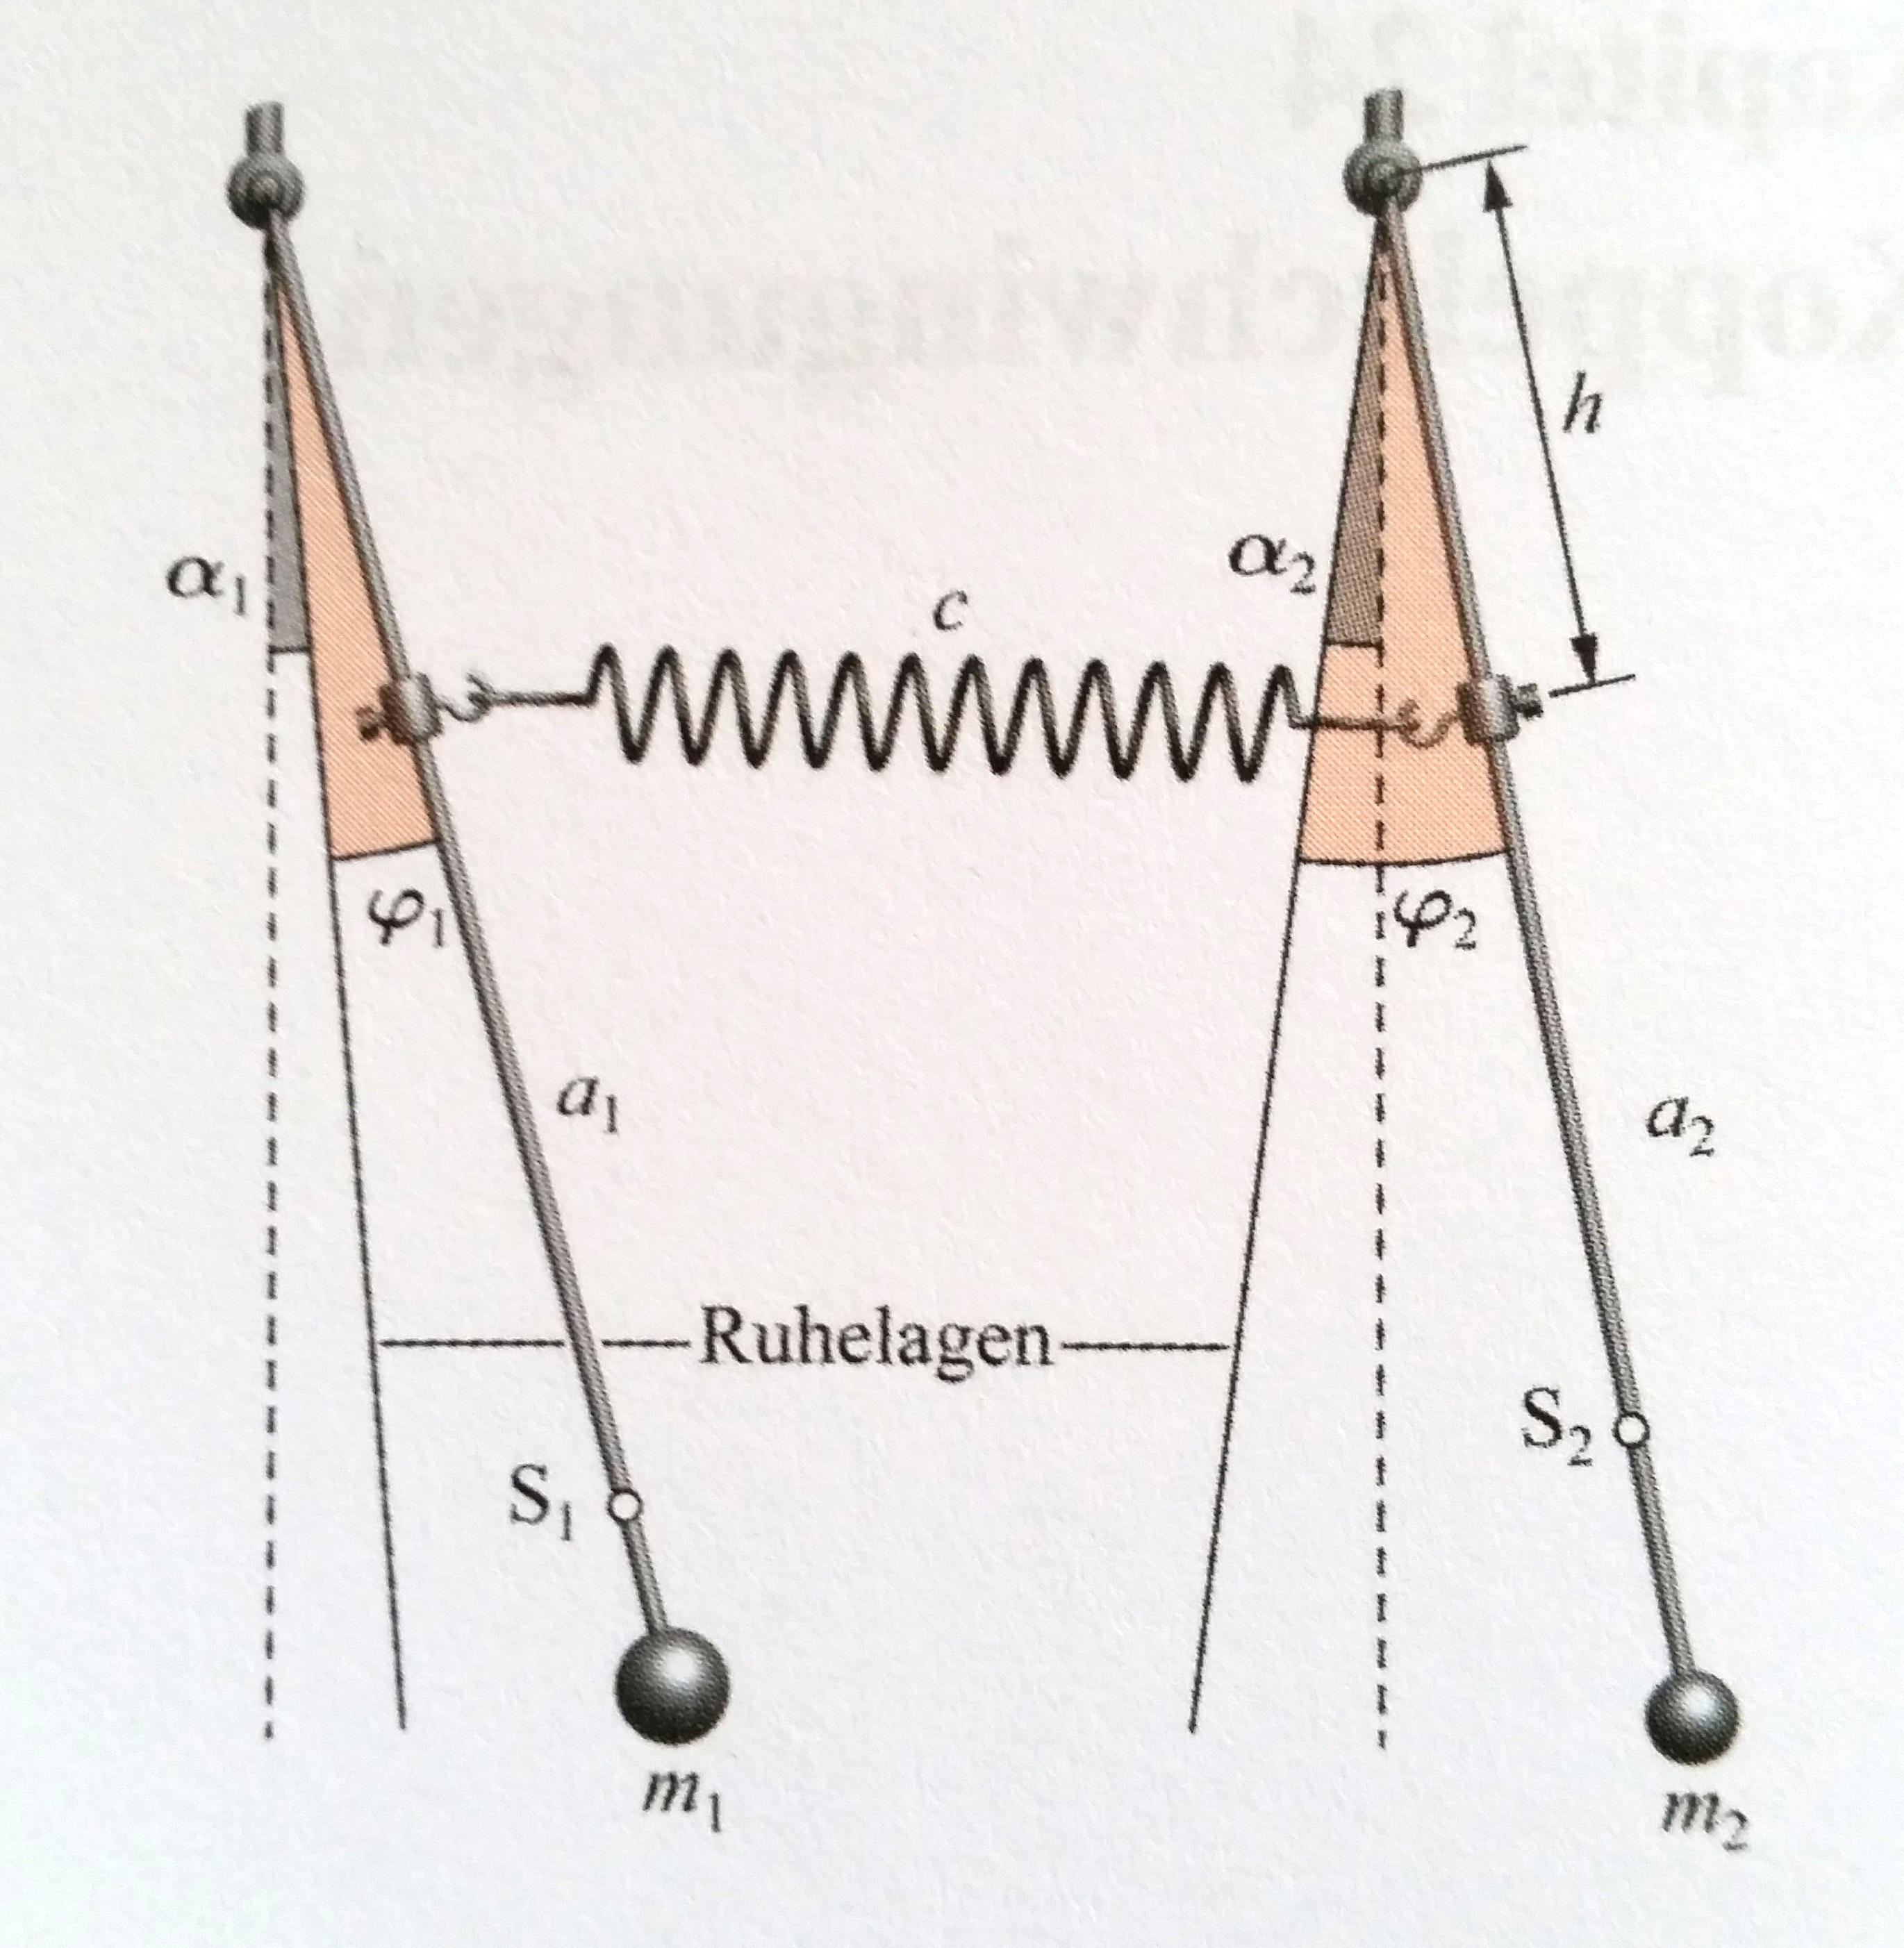
\includegraphics[width = 0.99\textwidth]{bilder/kopppendel.jpg}
\begin{itemize}
\itemsep0em
\item $J =$ Trägheitsmomente
\item $\alpha =$ Ruhelagewinkel
\item $a = $ Abstand vom Schwerpunkt zum Drehpunkt
\item $\varphi = $ Winkel gemessen ab der Ruhelage
\item $h = $ Abstand der Federbefestigung zum Drehpunkt
\item $l_0 =$ Verlängerung der Feder in Ruhelänge
\item $cl_0 = $ Vorspannung der Feder in Ruhelage
\item $A_s, A_D, \varphi_S, \varphi_D$ Aus Anfangsbedingungen
\end{itemize}
\end{minipage}

\end{document}
